% =====================================================================
% Experimental Astronomy (Springer) journal layout -- EMULATED.
% Compile with XeLaTeX (e.g. latexmk -pdfxe).
% Auto-generated from the NIM-A elsarticle source by build_ea_format.py;
% only the journal FORMAT changed -- text, figures, tables, and references
% are carried over verbatim from balloon511_nima_draft_zh.tex.
% For submission, replace this emulated preamble with the official Springer
% Nature class (sn-jnl.cls); the structure is already aligned to it.
% =====================================================================
\documentclass[11pt]{article}
\usepackage[a4paper,top=2.4cm,bottom=2.5cm,left=2.0cm,right=2.0cm]{geometry}
\usepackage{amsmath,amssymb}
\usepackage[UTF8]{ctex}
\usepackage{fontspec}
\setmainfont{TeX Gyre Termes}
\usepackage{booktabs}
\usepackage{graphicx}
\usepackage{pdflscape}
\usepackage[section]{placeins}
\graphicspath{{./}}
\renewcommand{\topfraction}{0.92}
\renewcommand{\bottomfraction}{0.8}
\renewcommand{\textfraction}{0.07}
\renewcommand{\floatpagefraction}{0.75}
\usepackage{xcolor}
\usepackage{tikz}
\usetikzlibrary{arrows.meta,positioning}
\usepackage{caption}
\captionsetup{font=small,labelfont=bf}
\usepackage{titlesec}
\titleformat{\section}{\normalfont\large\bfseries}{\thesection}{0.6em}{}
\titleformat{\subsection}{\normalfont\normalsize\bfseries}{\thesubsection}{0.5em}{}
\titleformat{\subsubsection}{\normalfont\normalsize\bfseries}{\thesubsubsection}{0.5em}{}
\titlespacing*{\section}{0pt}{1.3ex plus .2ex minus .2ex}{0.6ex}
\titlespacing*{\subsection}{0pt}{1.0ex plus .2ex minus .2ex}{0.5ex}
\usepackage{fancyhdr}
\pagestyle{fancy}
\fancyhf{}
\fancyhead[L]{\small\itshape Experimental Astronomy}
\fancyhead[R]{\small\thepage}
\renewcommand{\headrulewidth}{0.4pt}
\usepackage{cite}
\usepackage{hyperref}
\hypersetup{hidelinks}
\setlength{\emergencystretch}{3em}
\newcommand{\keV}{\,\mathrm{keV}}
\newcommand{\MeV}{\,\mathrm{MeV}}
\newcommand{\cms}{\,\mathrm{cm^{-2}\,s^{-1}}}
\newcommand{\phcms}{\,\mathrm{ph\,cm^{-2}\,s^{-1}}}
\newcommand{\cps}{\,\mathrm{s^{-1}}}
\newcommand{\wii}{W_{511}}
\newcommand{\aeff}{A_{\mathrm{eff}}}
\newcommand{\fzero}{F_{0}}
\newcommand{\fthree}{F_{3\sigma}}

\begin{document}
\thispagestyle{fancy}
\begin{flushleft}
{\LARGE\bfseries 气球载 511 keV Laue 透镜 TES 望远镜本底和未分辨线灵敏度的探测器耦合 Monte Carlo 估计 \par}
\vspace{1.1em}
{\large 作者信息暂隐\par}
\vspace{0.3em}
{\normalsize\itshape 单位信息暂隐\par}
\end{flushleft}
\vspace{0.7em}
\noindent\rule{\textwidth}{0.4pt}
\vspace{0.5em}

\noindent\textbf{摘要}\hspace{0.7em}本底决定气球载 511 keV Laue 透镜--过渡边缘传感器（TES）微量热计望远镜的灵敏度。本文建立一条端到端 Geant4/MEGAlib 模拟链，在同一个探测器--低温系统几何中输运聚焦信号、全部八类瞬发粒子族、按产生位置抽样的活化衰变和显式大气 511 keV 线，并统一施加 $510.58$--$511.42\keV$ 能窗、主动反符合及拓扑/视场选择。质量完备参考几何的瞬发加延迟诊断本底为 $(4.643\pm0.543)\times10^{-2}\cps$；该不同口径的数值用于定位来源，不作为屏蔽增益的同口径比较。正电子和中子贡献瞬发分量的 $96.8\%$，26 条选后延迟记录中有 24 条来自冷铜结构中的 $^{64}$Cu，另 2 条来自 $^{61}$Cu。该粒子与材料分解直接导向最终方向分级 BGO 屏蔽：侧、底、顶分别采用 40、30 和 10 mm 主动覆盖，同时保留侧入射光学孔径。逐像素施加 420 eV FWHM 能量响应后，最终全链的主动 veto 将瞬发率由 $2.849\times10^{-2}$ 降至 $4.072\times10^{-3}\cps$；第 15 天参考状态下的完整八族选择在大气层顶 $10^{-4}\phcms$ 参考流量下给出本底率 $6.965\times10^{-3}\cps$ 和信号率 $9.862\times10^{-4}\cps$。固定 $45^\circ$ 仰角的 20 d 轨迹折叠给出中心计数显著度 15.20 和 $3\sigma$ 流量阈值 $1.974\times10^{-5}\phcms$；条件式逐分量输运计数端点对应 5.67 和 $5.293\times10^{-5}\phcms$。本工作把可追溯的本底来源直接连接到最终屏蔽结构和任务尺度性能。

\vspace{0.7em}
\noindent\textbf{关键词}\hspace{0.7em}伽马射线仪器 $\cdot$ 511 keV 湮灭线 $\cdot$ 过渡边缘传感器微量热计 $\cdot$ Laue 透镜 $\cdot$ 气球载望远镜 $\cdot$ Monte Carlo 本底模拟

\vspace{0.3em}
\noindent\rule{\textwidth}{0.4pt}
\vspace{1.0em}

\section{引言}
\label{sec:intro}

银河系 511 keV 湮灭辐射是研究银河系正电子产生、传播和湮灭环境的重要观测探针。其谱学特征包括接近 511 keV 的双光子谱线和位于较低能量处的正电子素连续谱。正电子可与电子直接湮灭，或先形成对位正电子素并产生两个约 511 keV 光子；正交正电子素则通过三光子衰变形成连续谱。因此，谱线强度、轮廓和正电子素连续谱可以约束正电子减速和湮灭所在介质的性质 \cite{Prantzos2011,Jean2006}。在近似稳态假设下，INTEGRAL/SPI 测得的银河系 511 keV 总通量对应约几 $\times10^{43}\,\mathrm{e^+\,s^{-1}}$ 的正电子湮灭率 \cite{Prantzos2011,Kierans2020}。候选正电子来源包括恒星爆发中合成的 $\beta^+$ 不稳定核素、能够产生正负电子对的致密天体，以及更具推测性的粒子物理情景，例如由轻质量暗物质湮灭或衰变注入低能正电子。现有观测尚不能唯一确定其中的主导贡献 \cite{Prantzos2011,Siegert2016AA,Siegert2016V404}。

过去的宽视场观测已经建立了 511 keV 辐射的弥散形态。INTEGRAL/SPI 显示出明亮的中心核球成分和较弱的银盘成分，20 年数据分析进一步重建出中心、宽核球与银盘结构，但额外关联结构的证据仍较边际 \cite{Knodlseder2005AllSky,Siegert2016AA,Yoneda2025}。COSI 2016 年气球飞行独立探测到核球信号，并给出辐射比单一点源更延展的迹象 \cite{Kierans2020,Siegert2020COSI}。谱学测量还约束了湮灭介质的物理状态和运动学：SPI 谱线可分解为约 $1.3\keV$ FWHM 的窄成分和约 $5.4\keV$ 的宽成分，并已在银河系内区搜寻其中心能量与线宽的变化 \cite{Jean2006,Siegert2019Kinematics}。然而，511 keV 天图记录的是正电子减速并湮灭后的位置，不一定是正电子最初产生的位置；正电子在热化之前可在磁化的多相星际介质中传播。因此，现有弥散形态和谱学约束仍不能单独判定主导来源，或还原湮灭前的输运历史 \cite{Prantzos2011}。

宽视场康普顿和编码孔径仪器非常适合测量核球和银盘的总体发射。为了检验中心区域是否还包含未分辨中心增强、紧致源或可测量的谱线运动学结构，需要一种互补的定点仪器。探测到点状或窄集中分布的特征，将表明部分湮灭在空间上是局域的；未探测到信号则会限制紧致成分，但不能排除正电子逃逸后以弥散形式湮灭的源族。INTEGRAL/IBIS 紧致源搜索未发现银河系 511 keV 点源，并针对银河系中心方向约 10 Ms 的曝光给出约 $1.6\times10^{-4}\phcms$ 的 $2\sigma$ 上限 \cite{DeCesare2011}。该上限既给出了以往紧致源搜索的比较尺度，也构成新型窄视场定点仪器的灵敏度目标。

Laue 光学利用透射式 Bragg 衍射，将来自已知方向的光子聚焦到小型焦面上，为这种定点观测提供了一种途径 \cite{Barriere2009Laue,Barriere2011LauePrototype}。当探测器相关本底占主导时，把大口径收集的通量汇聚到较小的灵敏探测器面积上，可以提高点源灵敏度 \cite{Weidenspointner2006MAX}。相应的焦面必须兼具窄能量响应和足够的 511 keV 阻止效率。过渡边缘传感器（transition-edge sensor, TES）微量热计利用超导体陡峭的电阻转变测量沉积能量引起的微小温度变化，可在 511 keV 处提供亚 keV 能量分辨率 \cite{Shirazi2023,Zhang2022TESGamma}。阵列用于覆盖焦斑，厚吸收体与多层布局则提高全能量效率。Laue 聚焦压缩接收相空间，而 TES 响应允许使用窄线窗并进行精细谱线轮廓测量。所得仪器以视场换取集中束流和高分辨率谱学能力，是对核球和银盘宽视场测量的补充，而不是替代。

不过，TES 探测器本征的高能量分辨率和聚焦光学的聚焦性能并不足以单独论证整套探测系统针对点源的高分辨率 \cite{Shirazi2023,Hu2026}。大气环境中的宇宙线本底在探测器灵敏区沉积的瞬发本底谱，以及宇宙线在探测器及探测器周围物质活化引起的次级延时本底谱，也会影响探测系统对于科学源探测的分辨能力 \cite{Gallego2025Balloon,Tian2026DIXE}。

本工作旨在量化球载 Laue 透镜--TES 阵列望远镜系统在高空环境下对于银河系中心 511 keV 点源的探测性能，同时研判本底的来源与分布，给出进一步设计优化的指导意见。

\subsection{科学目标与仪器要求}
\label{sec:requirements}

\begingroup
\clubpenalty=10000
\widowpenalty=10000

本文模拟的仪器旨在探测此前仪器尚未发现的银河系中心区域 511 keV 点源或未分辨中心超额成分。INTEGRAL/SPI 测量表明，511 keV 天空辐射以弥散的核球和银盘发射为主 \cite{Siegert2016AA,Yoneda2025}。De Cesare 针对 INTEGRAL/IBIS 开展的紧致源专项搜索未发现银河系 511 keV 点源，并给出了银河系中心方向 10 Ms 曝光下的 $2\sigma$ 上限 \cite{DeCesare2011}。为与本文报告的 $3\sigma$ 灵敏度进行比较，我们在高斯近似下对该已发表上限作线性换算，得到基于 IBIS 结果的 $3\sigma$ 等效大气层顶上限 $2.4\times10^{-4}\phcms$。在飞行第 15 天的高度，保留的垂直剩余大气柱深为 $3.461\,\mathrm{g\,cm^{-2}}$。对于本文设计的固定 $45^\circ$ 仰角仪器轴，平面平行近似下的斜程柱深为 $4.895\,\mathrm{g\,cm^{-2}}$；采用与 NIST XCOM 在 511 keV 附近数据一致的有效干空气衰减系数 $0.08736\,\mathrm{cm^2\,g^{-1}}$，得到透过率 $T_{15,45}=0.6520$。施加该透过率后，定义唯一的载荷平面观测参考通量 $F_{0,\mathrm{ref}}=(2.4\times10^{-4})\times0.6520=1.565\times10^{-4}\phcms$。该参考通量将作为后文评估所模拟望远镜系统在可接受飞行时间内最小可分辨通量性能的参照。与 INTEGRAL 已开展的宽视场光谱和编码孔径搜索相比，本文模拟的载荷引入 Laue 聚焦以改善点源响应，并采用高能量分辨率、多层厚吸收体 TES 微量热计阵列作为焦面探测器，以提高 511 keV 谱线测量能力 \cite{Shirazi2023,Caputo2017}。

本工作首先考虑早期测试用的气球载荷平台，并期望后续拓展到卫星观测平台。

\begingroup
\interlinepenalty=10000
这一目标对仪器和模拟提出四项要求。第一，望远镜必须将大口径透镜收集的 511 keV 光子汇聚到小型焦面上，从而提高聚焦光学的集光面积与探测器灵敏面积之比；这是一种窄视场定点构型，而不是扩大天空覆盖范围的手段。第二，焦面探测器必须具备足以分辨精细谱线结构的亚 keV 能量响应。第三，探测器和屏蔽模型必须抑制大气本底、活化本底及侧向入射本底。第四，模拟链必须一致处理瞬发本底、延迟活化、聚焦信号、veto、事例拓扑及任务时间变化，使信号和本底在相同的探测器选择条件下进行评估。
\par
\endgroup

本文余下结构如下：第 2 节给出探测器与低温系统质量模型；第 3 节描述模拟框架——模拟流程、光学耦合、本底来源、事例选择，以及任务时间轨迹折叠（第~\ref{sec:mission_time_fold}~小节）；第 4 节给出选后率和灵敏度结果以及归一化、收敛与边界检查；第 5 节为讨论与结论。

\endgroup

\section{探测器与低温系统质量模型}
\label{sec:geometry}

本文采用本项目早期设计的一套通用质量模型模板。该模型包含安装在小型稀释制冷机（DR）冷端的气球载 TES 多层阵列，以及各级冷盘与热屏蔽、磁屏蔽与被动屏蔽、侧入射窗口、准直器、铜热连接、主动闪烁体和低温服务结构 \cite{Shirazi2023,Gottardi2021TESReview}。图~\ref{fig:mass_model} 给出了该质量模型模板的示意图；定量计算则区分下文所述的初始 CsI 参考几何和最终 BGO 几何。

TES 探测器概念采用本实验室研发的 AlMn 薄膜与吸收体耦合结构。AlMn 合金的相变温度可通过成分和退火工艺调节，适于阵列制备，并且对磁场相对不敏感 \cite{Xie2026AlMn,Vavagiakis2017AlMnMagnetic}。在本文概念设计中，TES 温度计为厚约 $200\,\mathrm{nm}$、名义 Mn 原子浓度为 $2000\,\mathrm{ppm}$ 的 AlMn 薄膜，而 $\gamma$ 射线吸收体为毫米量级金属体。吸收体采用 $1.5\times1.5\times3.0\,\mathrm{mm^3}$ Ta 像素；Ta 的高原子序数提高了 511 keV 光子的相互作用效率。在 511 keV 处，单层 $3.0\,\mathrm{mm}$ Ta 的预估相互作用效率约为 $49\%$，相应的六层效率接近 1。当前几何中，相邻 Ta 阵列层的中心间距为 $12\,\mathrm{mm}$；该间距的设计兼顾后续基于康普顿运动学轨迹重建的 veto 机制。选择 Ta 还考虑了其作为超导体在低温下较低的体积热容（本文采用 $10^{-2}\,\mathrm{J\,K^{-1}\,m^{-3}}$ 的量级估计）及其较高的光电--康普顿相互作用比。根据 NIST XCOM 在 511 keV 附近的截面，该比值约为 0.731 \cite{NISTXCOM}。在探测器响应模型中，我们根据本实验室已开发的 X 射线 TES 的实验经验 \cite{Xie2026AlMn}，采用 $\Delta E_{\mathrm{FWHM}}\simeq420\,\mathrm{eV}$ 作为 511 keV 处的预估能量分辨率和探测器响应后处理输入。

由于 TES 薄膜与 Ta 吸收体在尺寸和质量上相差很大，且 TES 薄膜本身对 511 keV 光子的相互作用贡献可忽略，输运几何使用 Ta 吸收体代表 TES 像素的主要敏感体积。显式建模的敏感体积共 6 层，每层包含 376 个 Ta 吸收体像素，总计 2256 个像素；每个像素长、宽均为 $1.5\,\mathrm{mm}$，厚度为 $3\,\mathrm{mm}$。每个 Ta 像素下方放置一个 Si 衬底代理；由于本模拟不处理详细热传导，使用 Si 代表 $\mathrm{SiO_2}$--$\mathrm{SiN_x}$--Si 衬底。TES 薄膜、布线和读出细节不作为显式相互作用体积逐层建立，而是通过假设的能量响应和服务质量代理进入模型。与响应 FWHM 独立定义，保留的 W2 分析选择采用 511 keV 线窗 $W_{511}=511\,\mathrm{keV}\pm420\,\mathrm{eV}$，即 $510.58$--$511.42\,\mathrm{keV}$。

TES 阵列安装在铜支架和热连接上；铜热指从样品盒后端穿出并连接 50 mK 冷盘。近场样品盒采用 2 mm Nb 内层和 2 mm MuMetal 外层，MuMetal 在材料表中按 Ni:Fe = 4:1 近似。沿光路依次放置各级 $300\,\mu\mathrm{m}$ Al 热屏蔽窗、$25\,\mu\mathrm{m}$ Be 真空窗和与 TES 像素对准的 $8\,\mathrm{mm}$ W 多孔准直器；这些侧入射开口均由贯穿周围壳层的布尔切口生成。初始参考几何在侧壁和端面使用分段 CsI，最终优化版本将这层外部主动屏蔽替换为 BGO。整个仪器框架旋转 $45^\circ$，使局部侧窗在天顶参考坐标中向上倾斜 $45^\circ$。

在最终闪烁体主动 veto 计算中，主动屏蔽体积内的能量沉积在后处理中按事例汇总。统一的探测器层反符合选择随后施加 $50\keV$ 的闪烁体离线沉积能 veto 阈值；屏蔽总沉积达到或超过该阈值的事例被 veto。

\begin{figure}[t]
\centering
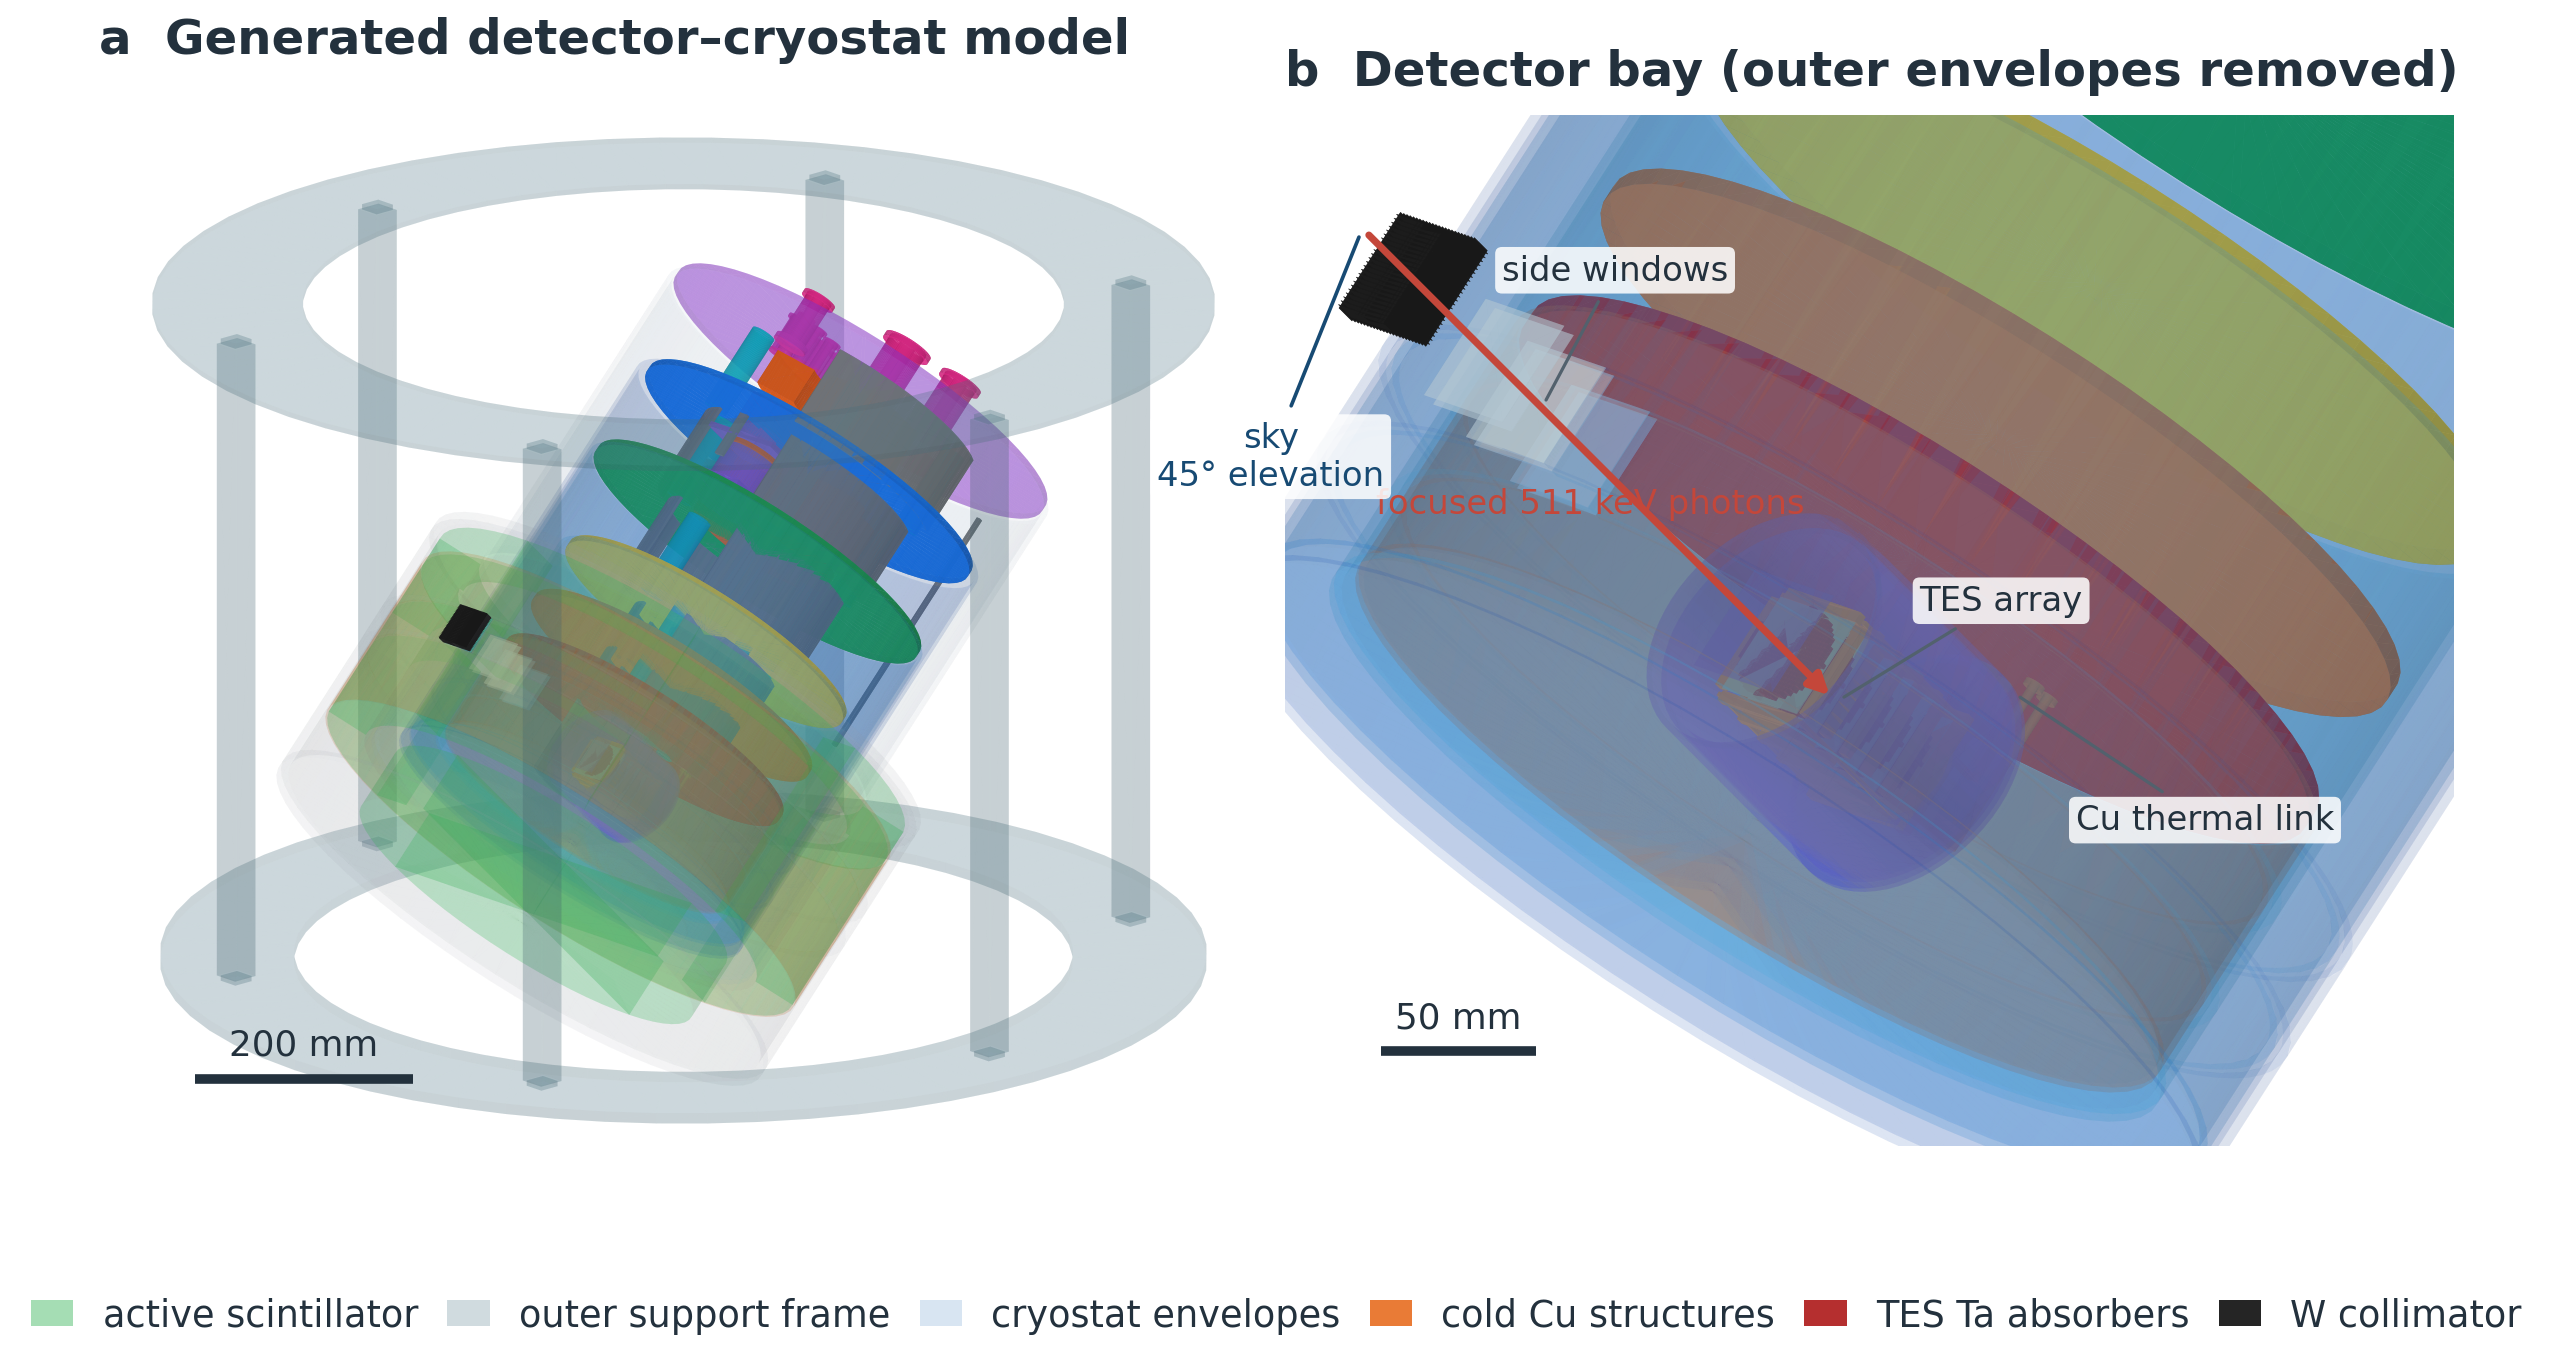
\includegraphics[width=0.98\linewidth]{paper_source_figure_table/fig_reference_detector_cryostat_geometry.png}
\caption{本项目早期设计的通用探测器--低温系统质量模型模板示意图。（a）模板总体视图，包括外部支撑框架、主动闪烁体屏蔽、低温级和服务结构。（b）隐藏外部包络后的探测器舱视图，显示 TES Ta 阵列、铜热连接、侧窗组和 W 准直器。孔径轴取 $45^\circ$ 仰角；红箭头表示聚焦 511 keV 光子从朝天准直器到 TES 阵列的名义传播路径。部分外层为清晰显示而设为半透明。}
\label{fig:mass_model}
\end{figure}

\FloatBarrier

\section{模拟框架}
\label{sec:framework}

本文采用基于详细质量模型的探测器耦合 Monte Carlo 输运，计算 511\,keV 谱仪的响应与本底 \cite{Sturner2003}。图~\ref{fig:workflow} 将端到端计算按物理来源分为三条分支：聚焦信号、瞬发大气本底和延迟活化本底。Laue 光学系统与探测器--低温系统分别建立质量模型。参考点源首先在 Laue 透镜模型中输运；到达焦平面的光子位置与方向写入 MEGAlib EventList，并据此初始化探测器侧 Monte Carlo 输运。对于每一版设计，聚焦信号输入与全部本底源均在第~\ref{sec:geometry}~节所述的同一完整探测器--低温系统质量模型中输运。

宽带瞬发输运与活化产生输运采用同一套 EXPACS/PARMA 大气辐射场定义，并作为并行计算执行。瞬发分支包含两个独立模拟的输入：EXPACS/PARMA 给出的宽带伽马射线连续谱与粒子场，以及独立构建的单能大气正电子湮没 511\,keV 线源。后者的参考归一由已发表的大气测量结果约束 \cite{Mahoney1981Atmospheric,Harris2003Atmospheric}。本文单独输运该线源，是因为所用 EXPACS/PARMA 光子表在 511\,keV 处只有连续谱插值，而没有独立的谱线条目。在延迟活化分支中，BUILDUP 输运记录核素产额、材料体积和产生位置。这些记录用于计算飞行期间积累的活度并构建参考时刻核素清单；随后按记录的产生位置抽样延迟衰变，并在探测器--低温系统模型中输运。

聚焦信号、宽带瞬发本底、大气 511\,keV 线和延迟活化四类探测器侧事例目录统一施加相同的探测器响应、主动 veto 判据与 Compton 拓扑检验。选后本底事例按入射粒子族、母核素和产生体积分解，并据此定义和筛选候选屏蔽几何。最终候选几何固定后，再将其选后信号率与分量本底率沿任务时间及所采用的参考轨迹进行解析折叠，以计算累计计数和未分辨线灵敏度。多日飞行会采样变化的大气与地磁条件，因此该折叠并非将单一 Monte Carlo 快照按飞行时间简单缩放；其定义和多点直接输运检验见第~\ref{sec:mission_time_fold}~小节。图~\ref{fig:workflow} 末端的设计反馈节点表示利用任务尺度评价约束后续屏蔽改进，并不表示本文的任务折叠先于所用最终候选几何的定义与输运。下文依次给出源模型、输运归一化、事例选择判据和轨迹计算方法。

\begin{landscape}
\centering
\vspace*{\fill}
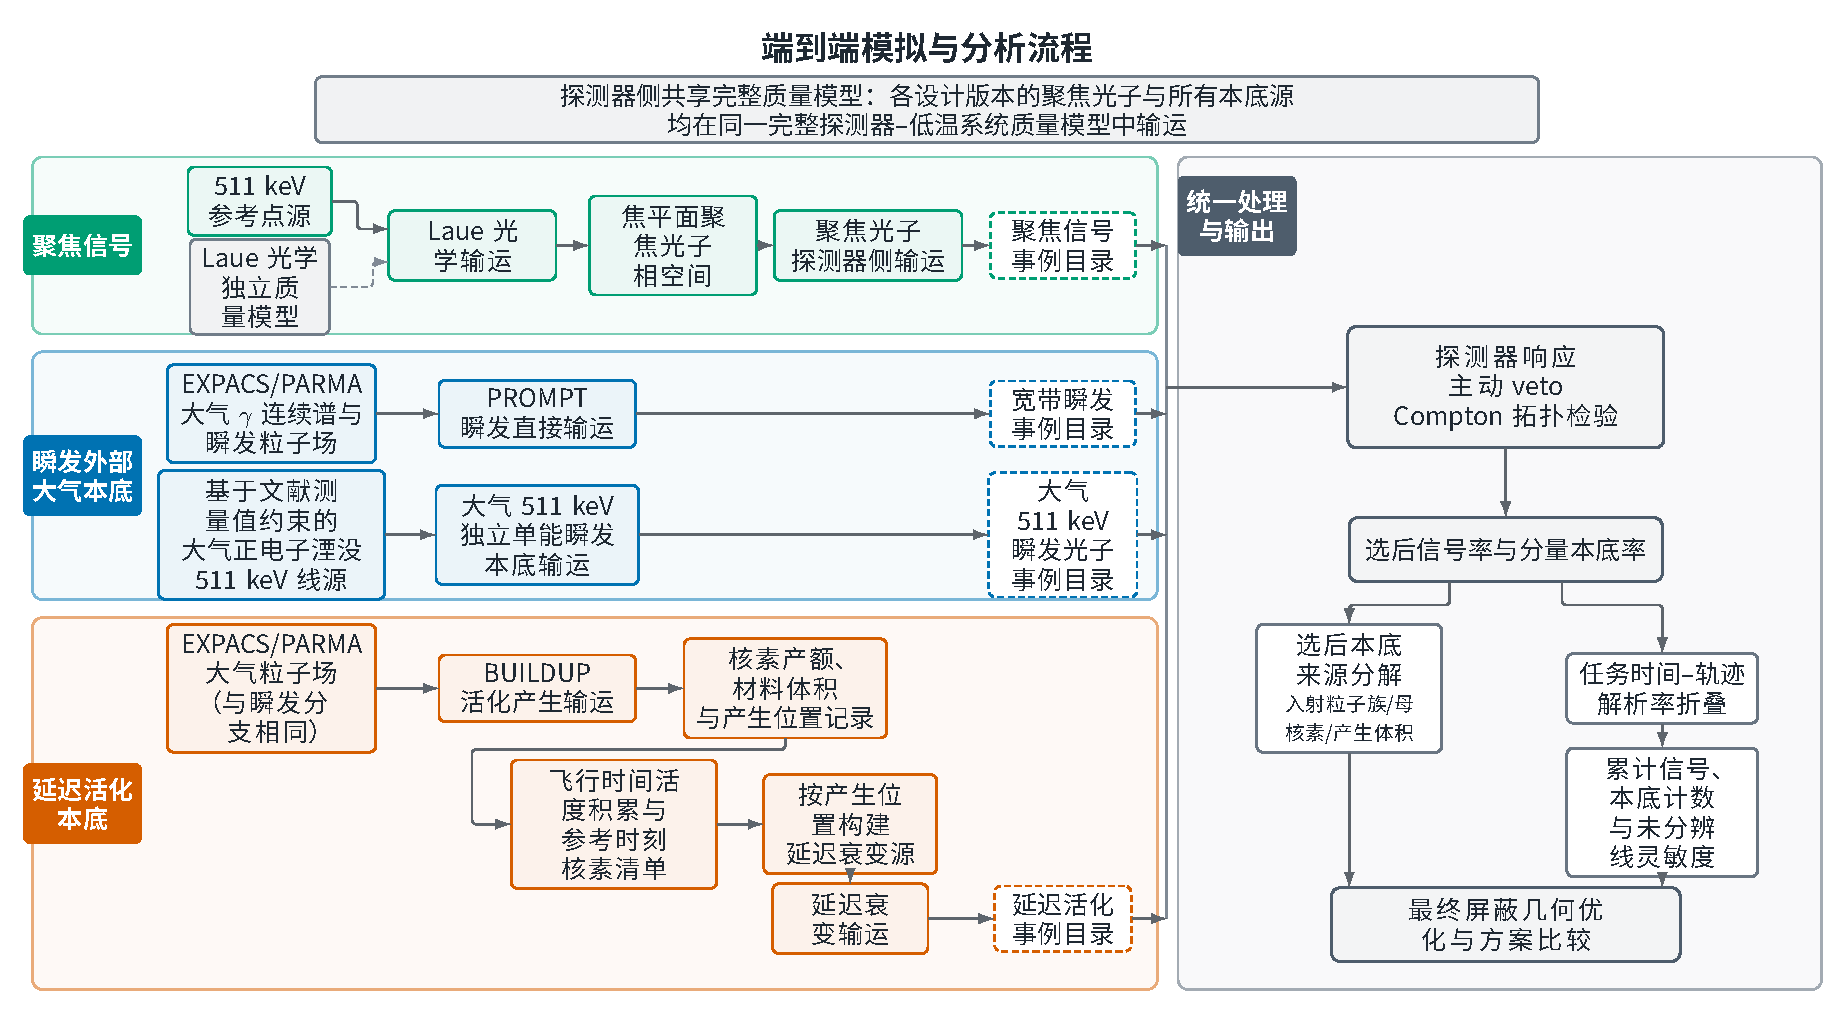
\includegraphics[width=0.94\linewidth]{paper_source_figure_table/fig_simulation_workflow_m04_zh_20260810.pdf}
\captionof{figure}{端到端模拟与分析流程。三条物理分支生成四类探测器侧事例目录：聚焦信号、宽带瞬发本底、大气 511\,keV 瞬发线和延迟活化本底。各事例目录统一施加探测器响应、主动 veto 和 Compton 拓扑检验。选后本底来源分解用于候选几何筛选；本文报告的任务折叠随后针对已固定的最终候选几何进行。末端节点表示任务尺度结果对后续方案比较和屏蔽改进的反馈。}
\label{fig:workflow}
\vspace*{\fill}
\end{landscape}

\FloatBarrier

\subsection{Laue 光学与探测器耦合信号输运}
\label{sec:optics}

本文模拟采用基于镶嵌型 Ge(111) 晶体的 Laue 透镜系统 \cite{Barriere2009Laue,Barriere2011LauePrototype}，通过光学设计实现 $10\,\mathrm{m}$ 的焦距、511 keV 单环参考响应，以及 511 keV 下 $20.1\,\mathrm{cm^2}$ 的有效面积；有效面积按
\begin{equation}
  A_{\mathrm{eff}}(E)=A_{\mathrm{inc}}\frac{N_{\mathrm{fp}}(E)}{N_{\mathrm{inc}}(E)}
  \label{eq:laue_aeff}
\end{equation}
计算，其中 $A_{\mathrm{inc}}$ 为蒙特卡洛入射采样面积，$N_{\mathrm{inc}}(E)$ 为入射光子数，$N_{\mathrm{fp}}(E)$ 为满足聚焦/焦面截取条件的光子数。
采用镶嵌晶体系统是为了在满足预期设计聚焦性能的同时便于蒙特卡洛计算；实际工程适配时也可考虑其他候选方案。

Laue 光学分支用于计算聚焦性能，并显式输运信号光子穿过 Ge 晶体质量。

为此,晶体对光子的衍射概率不再作为一个效率参数叠加给光子,而是在 Geant4 应用层定义为一个离散过程 \cite{Agostinelli2003,Allison2016}。该过程按当前光子相对晶面的角偏差取衍射概率 $R(|\Delta\theta|)$,并把它转换为一个有限的等效衍射平均自由程 $\lambda_{\mathrm{diff}}$,使光子穿过晶体路径 $\ell$ 时累计的衍射概率复现该值:$1-\exp(-\ell/\lambda_{\mathrm{diff}})=R(|\Delta\theta|)$,即 $\lambda_{\mathrm{diff}}=-\,\ell/\ln[1-R(|\Delta\theta|)]$;为避免与标准光电吸收重复计数,$R$ 先按未吸收份额归一($R/(1-A)$)再转成自由程。该自由程交回 Geant4 后,衍射过程与标准电磁过程(光电吸收、康普顿散射)在同一竞争框架下各自抽样相互作用长度,由最短者决定谁先发生,而不是在晶体边界强制拦截光子。未被抽中发生衍射的光子仍按标准电磁物理继续输运,可能被吸收、散射或直接透射。

衍射概率优先由外部 XOP/CRYSTAL rocking-curve map 按角偏差插值给出:该曲线由 XOP 工具包的 CRYSTAL/diff\_pat 模块(经 xoppylib 调用,以 DABAX 晶体学数据为输入)在预处理阶段一次性离线计算 \cite{SanchezDelRio2011XOP},给出 Ge(111) 反射率/透射率/吸收随角偏差的曲线;输运过程中对晶体内每一步实时计算角偏差,在该曲线上插值取当前衍射概率,即“库离线建表、概率随输运按角取用”。mosaic 取向通过对理想 Bragg 晶面法线施加高斯角扰动实现,扰动宽度由 30 角秒 mosaic FWHM 给出;衍射发生后,出射方向按扰动后的晶面法线镜面反射,光子能量不变。这种“过程类只负责输运接口、独立模型类负责概率与方向判定”的拆分方式,借鉴了 Geant4 中已有的晶体 Bragg 反射扩展工作的思路 \cite{Guan2023BraggReflection,Reiazi2025G4BraggReflection}，扩展到我们所需能段。

这里的参考信号是一个单色 511 keV 点源；其大气层顶取整参考尺度 $\fzero=10^{-4}\phcms$（见第~\ref{sec:requirements} 节）由 INTEGRAL/IBIS 的专门紧凑源上限提供依据，而非取自某个已观测天体 \cite{DeCesare2011}。信号以 MEGAlib 远场源方式构建 \cite{Zoglauer2006}，详细构建方式见第~\ref{subsec:pointsource} 节。信号经光学分支输运，记录的焦面穿越位置和方向被转换为 MEGAlib EventList，并作为探测器侧输运的输入。瞬发大气本底和活化衰变则分别在探测器--低温系统模型中独立引入。因此，光学分支仅提供聚焦信号相空间；统一响应与事例选择分析所用的信号和全部本底流均位于探测器侧分支。

\subsection{源构建}
\label{sec:background}

在上述三条物理分支内，本文独立构建四类探测器侧输入：参考点源的焦面 EventList、宽带瞬发大气场、单能大气 511\,keV 线，以及由活化核素清单构建的延迟衰变源。大气 511\,keV 线仍属于瞬发本底分支，活化产生与延迟衰变输运则作为两个独立阶段处理。该构建方式在施加共同探测器响应和事例选择前，保留了每类输入独立的归一化与来源追溯关系。

\subsubsection{瞬发大气源}
\label{subsec:prompt_source}

瞬发大气粒子场由 EXPACS/PARMA 给出。PARMA3.0 是由 PHITS 大气级联计算参数化得到、
并针对陆地宇宙线测量验证过的解析模型，EXPACS 是其公开表格与软件接口
\cite{Sato2015EXPACS,Sato2016PARMA4}。底层的粒子输运物理由 PHITS 提供：一次宇宙线
与大气核作用，次级强子、轻子、光子和中子在大气柱中继续输运，最终通量按海拔、
地磁截止刚度、太阳调制、能量和方向参数化。本文中 EXPACS/PARMA 给出随粒子种类、
动能、天顶角、地理位置、海拔、截止刚度和太阳活动变化的入射微分通量，且只用于构造
外部辐射场；探测器响应、反符合、拓扑选择和任务时间计数都在下游施加。参考源定义
采用纬度 $34^\circ$、经度 $100^\circ$、海拔 $38\,\mathrm{km}$、垂直截止刚度
$R_c=11.6\,\mathrm{GV}$，以及 2025-08-31 对应的太阳条件 $W=118.3$。

瞬发源包含光子、中子、电子、正电子、质子、$\alpha$ 粒子以及正负 $\mu$ 子。对每个
粒子族，EXPACS/PARMA 微分谱被转换为 MEGAlib 远场面积源，覆盖完整天顶角范围
$\theta=0^\circ$--$180^\circ$ 和完整方位角范围 $\phi=0^\circ$--$360^\circ$。天顶角
依赖用 20 个等 $\mu$ 微分分箱表示，其中 $\mu=\cos\theta$，每箱立体角
$\Delta\Omega=0.6283185307\,\mathrm{sr}$：前 10 箱为下行粒子，后 10 箱为上行或反照
成分。瞬发输运和活化产生输运都保留这两个半球，因此源构建阶段没有丢弃上行反照
粒子。图~\ref{fig:expacs_fullsphere_flux} 给出由源定义实际采用的全空间通量场。

\begin{figure}[t]
\centering
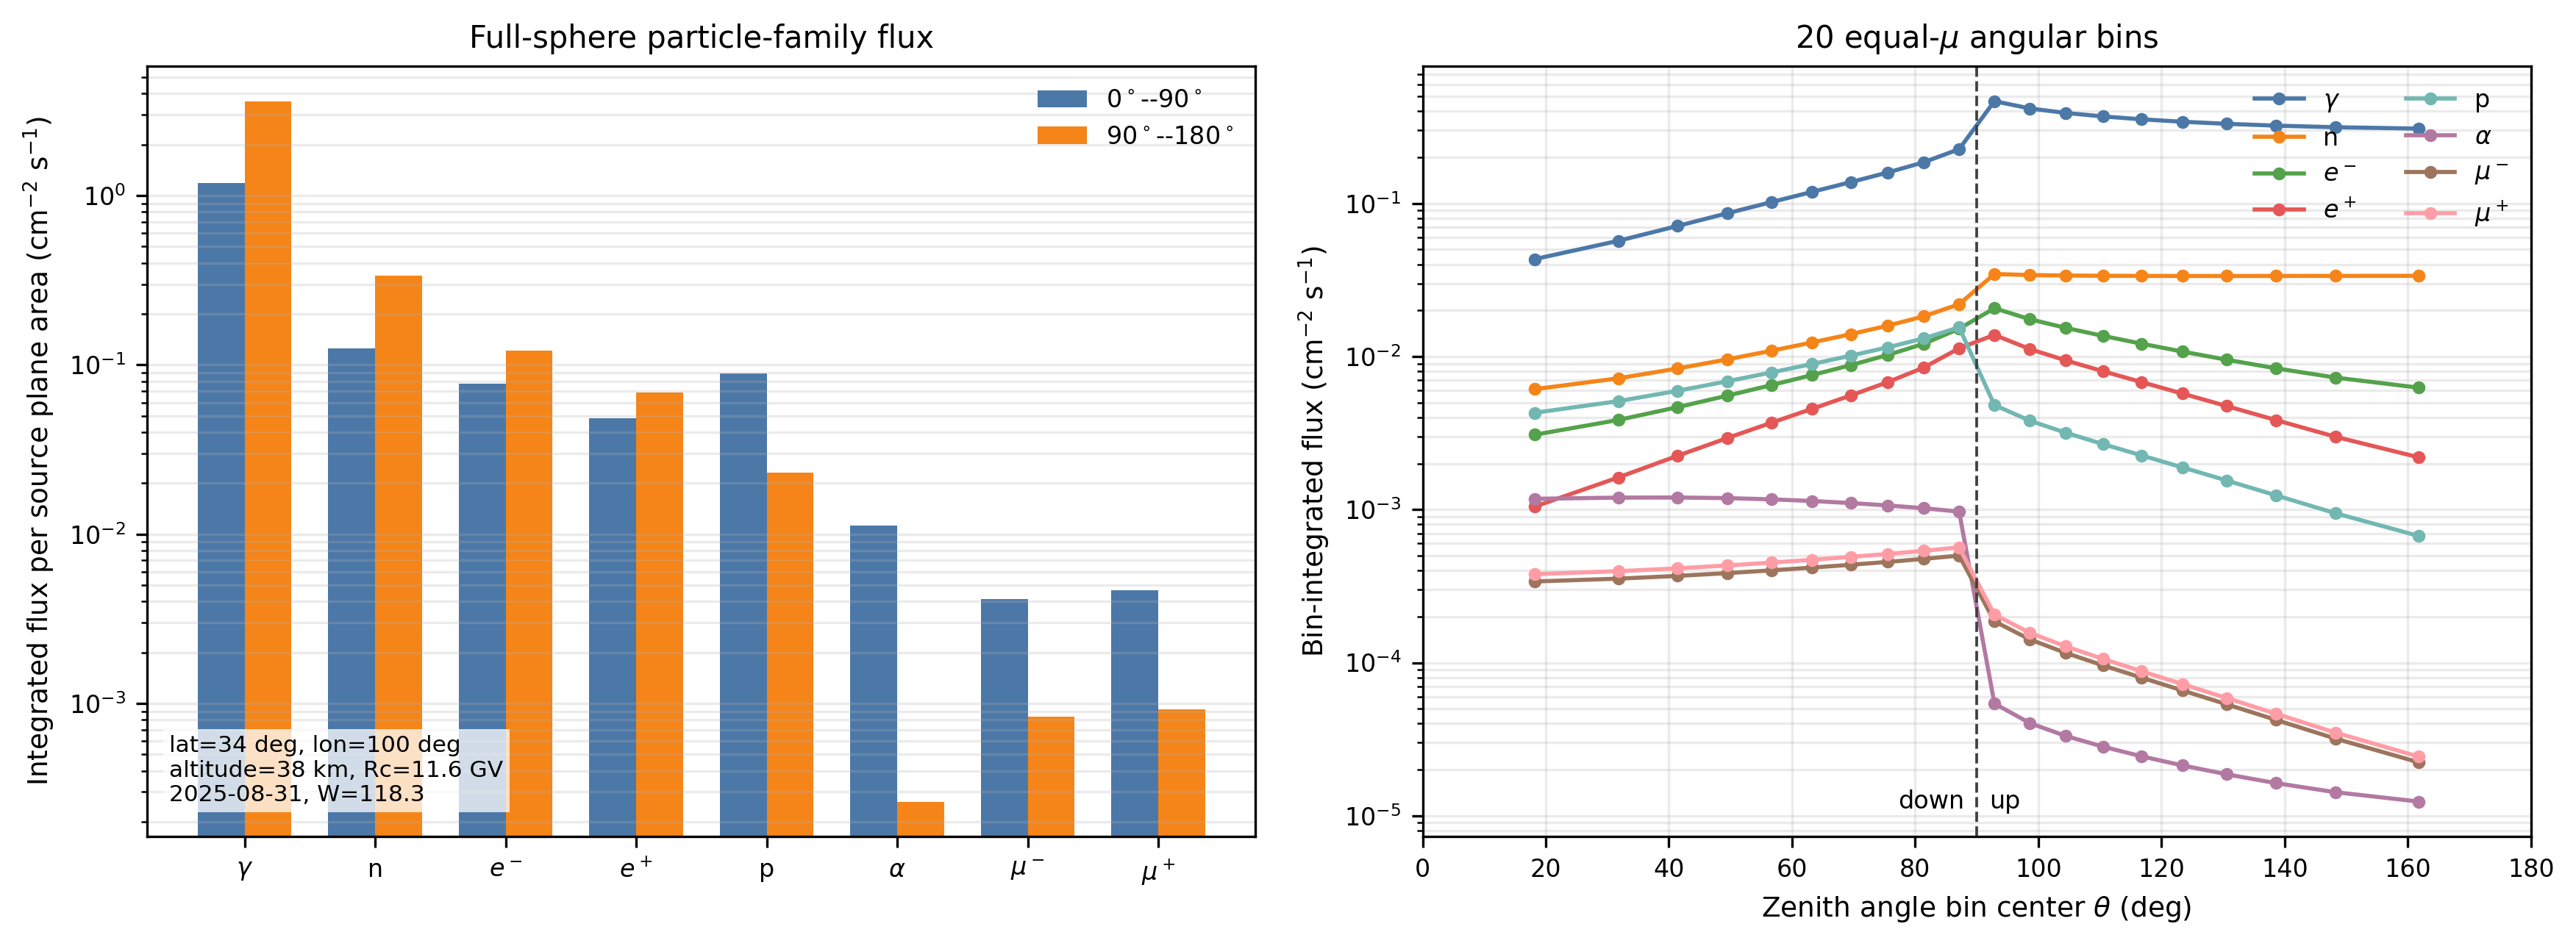
\includegraphics[width=\linewidth]{paper_source_figure_table/fig_expacs_fullsphere_flux.png}
\caption{用于生成瞬发和活化产生输运输入的 EXPACS/PARMA 全空间大气通量场。左：八类输运粒子族的能量和立体角积分通量，并按下行、上行半球分开。右：MEGAlib 远场源使用的 20 个等 $\mu$ 微分天顶角分箱的积分通量。该图直接由源定义输入表生成，环境参数为纬度 $34^\circ$、经度 $100^\circ$、海拔 $38\,\mathrm{km}$、$R_c=11.6\,\mathrm{GV}$、$W=118.3$。}
\label{fig:expacs_fullsphere_flux}
\end{figure}

积分源面通量约为 $4.80$、$0.462$、$0.199$、$0.117$、$0.112$、$0.0115$、$0.0050$
和 $0.0056\,\mathrm{cm^{-2}\,s^{-1}}$，分别对应 $\gamma$、$n$、$e^-$、$e^+$、$p$、
$\alpha$、$\mu^-$ 和 $\mu^+$；非光子成分合计约 $0.91\,\mathrm{cm^{-2}\,s^{-1}}$，
占全空间源面积分通量的 16\%。若严格按通量比例分配蒙特卡洛计数，这些少数粒子族的
探测器命中和活化统计将很差，因此非光子粒子族采用复制样本生成，再在率归一化中
去权重。随后所有粒子经 Geant4/MEGAlib 在探测器/低温系统质量模型中输运
\cite{Agostinelli2003,Allison2016,Zoglauer2006}；瞬发流和活化产生流各生成
25{,}210{,}216 个入射一次粒子。每个粒子种类用自身输运曝光归一：
\begin{equation}
  r_{\mathrm{event},j}=\left(\sum_i \mathcal{T}_{ij}\right)^{-1},
\end{equation}
其中 $\mathcal{T}_{ij}$ 为粒子种类 $j$ 在输运子样本 $i$ 中的曝光。由于光子流和
非光子流的采样与曝光结构不同，这种按种类归一是必要的；归一化检查要求每个种类满足
$r_{\mathrm{event},j}\sum_i\mathcal{T}_{ij}=1$，因此过采样只改变蒙特卡洛方差，
不改变物理期望率。

\subsubsection{大气 511 keV 线源}
\label{subsec:atm511_source_zh}

输运所用的 20 个 EXPACS/PARMA 大气光子表描述平滑连续谱。每个角分箱的能量网格均以
449.65 和 566.08\,keV 两个相邻表点夹住 511\,keV，因此 511\,keV 处的输入来自连续谱
插值，而不是独立的线节点。本文原样保留这些连续谱表，并另行输运在输入中建模为
511\,keV 单能的大气正电子湮没线；仪器展宽在后续探测器响应阶段施加。这种数值分离不能
证明平滑连续谱在物理上完全不含未解析的湮没辐射。潜在重叠被视为尚未量化的源模型
不确定度，而不预设为零。

该线源采用半经验模型。参考归一化、截止刚度因子和上行临边变暗形式参考了大气伽马射线
测量 \cite{Mahoney1981Atmospheric,Harris2003Atmospheric}；深度指数、半球通量比参数和
下行角分布核属于模型假设。全空间线积分通量写为
\begin{equation}
  \Phi_{4\pi}(X,R_c)=\Phi_{\mathrm{ref}}\,f_R(R_c)
  \left(\frac{X}{X_{\mathrm{ref}}}\right)^{\eta} f_{\odot},
  \label{eq:atm511_flux_zh}
\end{equation}
基线参数为 $\Phi_{\mathrm{ref}}=0.10\,\mathrm{ph\,cm^{-2}\,s^{-1}}$、
$X_{\mathrm{ref}}=3.6\,\mathrm{g\,cm^{-2}}$、$\eta=0.8$ 和 $f_{\odot}=1$；
截止刚度因子采用分段函数
\begin{equation}
 f_R(R_c)=
 \begin{cases}
  1.000, & R_c<7\,\mathrm{GV},\\
  0.805, & 7\le R_c<9\,\mathrm{GV},\\
  0.624, & 9\le R_c<11\,\mathrm{GV},\\
  0.532, & 11\le R_c<13\,\mathrm{GV},\\
  0.479, & R_c\ge13\,\mathrm{GV}.
 \end{cases}
 \label{eq:atm511_rigidity_zh}
\end{equation}
下行与上行通量之比及两个半球的积分通量为
\begin{equation}
  r_{\downarrow}(X)=\min\!\left[1,r_0
  \left(\frac{X}{X_{\mathrm{ref}}}\right)^{\beta}\right],\qquad
  \Phi_{\uparrow}=\frac{\Phi_{4\pi}}{1+r_{\downarrow}},\qquad
  \Phi_{\downarrow}=\frac{r_{\downarrow}\Phi_{4\pi}}{1+r_{\downarrow}},
  \label{eq:atm511_split_zh}
\end{equation}
其中 $r_0=0.20$、$\beta=0.5$。

这里 $\theta$ 为源天顶角：$\theta=0$ 表示光子来自天顶方向，$\theta=\pi$ 表示
来自下方的上行/反照光子。对上行半球，令 $\mu_{\uparrow}=-\cos\theta$，归一化临边变暗
分布为
\begin{equation}
  I_{\uparrow}(\mu_{\uparrow})=
  \frac{\Phi_{\uparrow}}{2\pi(1+a/2)}(1+a\mu_{\uparrow}),
  \qquad a=1.7 .
  \label{eq:atm511_upward_zh}
\end{equation}
对下行半球，令 $\mu_{\downarrow}=\cos\theta$，采用平板产生--逃逸核
\begin{align}
  K_{\downarrow}(\mu_{\downarrow},X)
    &=1-\exp\!\left[-\frac{X}{\Lambda_{511}\mu_{\downarrow}}\right],
    &\Lambda_{511}&=11.5\,\mathrm{g\,cm^{-2}},\quad 0<\mu_{\downarrow}\le1, \notag\\
  I_{\downarrow}(\mu_{\downarrow},X)
    &=\frac{\Phi_{\downarrow}}{2\pi\mathcal{A}(X)}
      K_{\downarrow}(\mu_{\downarrow},X),
    &\mathcal{A}(X)&=\int_0^1K_{\downarrow}(\mu,X)\,\mathrm{d}\mu .
  \label{eq:atm511_downward_zh}
\end{align}
在地平线方向采用连续极限 $K_{\downarrow}(0,X)=1$。该衰减尺度与 511\,keV 附近
干空气的质量衰减系数一致 \cite{NISTXCOM}。

全空间沿用瞬发源的 20 个等 $\mu$ 分箱，每个半球 10 个，$\Delta\mu=0.1$，且
$\Delta\Omega=2\pi\Delta\mu=0.628319\,\mathrm{sr}$。MEGAlib 在以 $(5,0,9)$\,cm
为中心、半径 60\,cm 的远场起始球所对应的投影圆盘上抽样入射位置；率归一化采用
$A_{\mathrm{proj}}=\pi R^2=1.13097\times10^4\,\mathrm{cm^2}$，而不是物理球面面积
$4\pi R^2$。大气线输运源卡采用的第 15 天代理状态为
$X=3.46147\,\mathrm{g\,cm^{-2}}$、$R_{c,\mathrm{line}}=11.0\,\mathrm{GV}$，由此得到 $\Phi_{4\pi}=0.0515559\,
\mathrm{ph\,cm^{-2}\,s^{-1}}$、$\Phi_{\uparrow}=0.0431028$ 和
$\Phi_{\downarrow}=0.00845307\,\mathrm{ph\,cm^{-2}\,s^{-1}}$。该蒙特卡洛输运生成
$3.0\times10^6$ 个光子，实际等效曝光为 5143.83\,s，单事例率权重为
$1.94408\times10^{-4}\,\mathrm{s^{-1}}$。用于瞬发和活化逐时缩放的状态相关 PARMA 场
在第 15 天取 $R_{c,\mathrm{PARMA}}=11.6\,\mathrm{GV}$。二者均位于
$11\le R_c<13\,\mathrm{GV}$，故使用相同的 $f_R=0.532$；任务折叠中的大气线分支仍沿用
其独立的代理刚度曲线。

\subsubsection{延迟活化源}
\label{subsec:delayed_source}

对于延迟模拟，则另行执行一个活化产生流，方法是在瞬发本底输运中打开 BUILDUP。活化
产生流不作为即时探测器本底计数，而是记录每个放射性产物的核素、材料体积和产生位置。
这些记录通过产生--衰变积累方程转换为固定到飞行过程中某一参考时刻的放射性群体，
基态半衰期已对照 NUBASE2020 校验 \cite{Kondev2021NUBASE}。对核素 $k$，
\begin{equation}
  A_k(t_{\mathrm{flight}}) = P_k\left[1-\exp\left(-\lambda_k t_{\mathrm{flight}}\right)\right],
  \qquad \lambda_k = \frac{\ln 2}{t_{1/2,k}},
\end{equation}
其中 $P_k$ 是由活化产生输运推得的产生率，参考状态取 $t_{\mathrm{flight}}=15\,\mathrm{d}$。
质量完备参考几何的延迟源构建使用固定延迟总活度 $141.83\,\mathrm{Bq}$。该数值继续作为下文本底来源比较的参考；最终方向分级构型使用另一套全八族清单与归一化。

位置信息并非只来自聚合后的同位素清单。标准清单记录产生体积和核素计数；产生位置
构建另在 MEGAlib 的 stepping-action 层加入自定义记录钩子：在活化积累模式中
每存入一个延迟核素，钩子就在同一时刻写出一条产生位置记录，包含逻辑体名称、
pre-step 位置 $(x,y,z)$、核素编号 $1000Z+A$、激发能、时间、过程和 track ancestry
信息。固定第 15 天群体随后按体积、核素和激发态与这些记录匹配，使延迟源能够使用
模拟产生坐标，而不是只有体积积分活度。参考探测器清单按产生体积、核素、入射粒子族、
材料类别和产生坐标汇总。这些量描述源构建而非探测器计数；延迟衰变经过共同几何和
共同事例选择输运后才施加探测器响应。

产生位置是否值得保留，可以直接用同一张产生表检验。延迟衰变在局部材料中发射，
下游衰减、主动屏蔽 veto 概率和事例拓扑都取决于核素产生在哪里；而不同入射粒子族
的能量损失、停止和俘获历史不同，其活化产物也不必落在相同的材料里。为量化这一点，
把加权产生行按入射粒子族和材料类别分组，用 total-variation 距离比较两个粒子族
$a$、$b$ 的活度归一化材料分布：
\begin{equation}
  D_{\mathrm{TV}}(a,b) =
  \frac{1}{2}\sum_c \left| f_{a,c} - f_{b,c} \right| ,
\end{equation}
其中 $f_{a,c}$ 为入射族 $a$ 在材料类别 $c$ 中产生的延迟活度占比。产生体积归入
主动 CsI、外部机械结构、冷板、被动钨/准直器、窗口、TES 和其他内部结构七类。体积积分源或
轴对称径向源可以保住总活度，却会抹掉这些入射族--材料--核素--坐标之间的相关性；
产生位置构建把它们保留在进入探测器输运之前的源里。

延迟衰变源因此从采样的产生位置发射，而不是从轴对称分布发射。设加权产生表第 $j$
行的活度权重为 $w_j$，总活度 $A=\sum_j w_j$。构建时以 $p_j=w_j/A$ 为概率有放回
抽取 $M$ 个产生位置，并给每个采样点源相同通量 $A/M$，则第 $j$ 行获得的期望活度为
\begin{equation}
  \mathbb{E}\!\left[N_j\frac{A}{M}\right] = M p_j \frac{A}{M} = w_j ,
\end{equation}
即该估计保持总活度，并对加权空间分布无偏。这里 $M$ 是等活度采样点源的数目，是
采样规模而不是物理产生行数。参考延迟源在源定义层面保持固定总活度，并在与瞬发流
相同的探测器/低温系统几何中输运；名义计算输运 $10^{6}$ 个延迟衰变，相应的 Cosima
live time 只是生成衰变序列的输运记录，不作为物理气球曝光时间使用。

表~\ref{tab:background_source_model} 汇总了当前探测器耦合计算使用的源层级。它放在
源模型部分，是因为这里定义的是入射粒子场和延迟放射性群体；探测器 veto 和拓扑选择
都在后续选择部分才施加。

\begin{table}[t]
\centering
\caption{当前探测器耦合链路中的本底源分层。表中只定义源构建；反符合、拓扑筛选和线窗在第~\ref{sec:selection} 节才施加。}
\label{tab:background_source_model}
\begin{tabular}{p{0.22\linewidth}p{0.34\linewidth}p{0.34\linewidth}}
\hline
层级 & 物理作用 & 当前实现 \\
\hline
瞬发大气输运 & 大气次级粒子造成的直接探测器命中 & EXPACS/PARMA 全空间源定义，环境为纬度 $34^\circ$、经度 $100^\circ$、海拔 $38\,\mathrm{km}$、$R_c=11.6\,\mathrm{GV}$、$W=118.3$；$\gamma$、$n$、$e^\pm$、$p$、$\alpha$ 和 $\mu^\pm$ 覆盖 20 个等 $\mu$ 微分天顶角分箱，并同时包含下行和上行半球；生成 25,210,216 个入射一次粒子。 \\
大气 511\,keV 线 & 与科学线在能谱上简并的大气正电子湮没光子 & 独立单能全空间分量，覆盖 20 个等 $\mu$ 分箱（每个半球 10 个）；第 15 天 $\Phi_{4\pi}=0.0515559\,\mathrm{ph\,cm^{-2}\,s^{-1}}$；生成 $3.0\times10^6$ 个光子，实际等效曝光 5143.83\,s。 \\
活化产生 & 放射性核素产生及其产生位置历史 & 在瞬发本底输运中打开 BUILDUP 得到活化产生流，同样保留两个半球和八类粒子族；生成 25,210,216 个入射一次粒子。 \\
固定延迟放射性群体 & 连续曝光后采用的第 15 天状态放射性活度 & 产生--衰变积累，并用 NUBASE 校验的基态半衰期修正；质量完备参考为 $141.83\,\mathrm{Bq}$，最终方向分级构型为 $36.4525153\,\mathrm{Bq}$。 \\
产生位置衰变输运 & 延迟衰变粒子从采样产生位置发射 & 从加权产生表得到等活度采样点源；最终构型对 7 个正活化族各输运 $10^6$ 个延迟触发，负电子族是有限累积零观测，不虚构输运曝光。 \\
\hline
\end{tabular}
\end{table}

该产生位置表示并非对每条产生行都建立一个采样点源。每个正活度族抽取
$M=50{,}000$ 个产生位置并输运 $10^6$ 个延迟触发；先核对活度守恒和源序列化，
再把同一实现传入探测器响应和事例选择。选后率及其核素/体积分解见
第~\ref{subsec:reference_background_results_zh}~小节。

上述 $141.83\,\mathrm{Bq}$ 全粒子族第 15 天清单用于判断质量完备参考几何的活化来源；其 26 条选后延迟记录仍为 24 条 $^{64}$Cu 和 2 条 $^{61}$Cu。最终方向分级屏蔽计算改用经 NUBASE 修正的全八族清单，第 15 天总活度为 $36.4525153\,\mathrm{Bq}$。其中 $\alpha$、$e^+$、$\gamma$、$\mu^-$、$\mu^+$、$n$ 和 $p$ 是完成延迟输运的 7 个正活化族；$e^-$（负电子）的有限 BUILDUP 样本未观察到产生，即有限累积零观测，因此中心延迟率为零，且不虚构输运曝光或 Garwood 边界。主响应在完整选择后保留 78 条延迟记录，按入射族为 1 条 $\alpha$、5 条 $\mu^-$、60 条 $n$ 和 12 条 $p$；其余正活化输运族为零条最终记录。

有限 $M$ 抽样构成源级边界，而不是泊松计数区间。主导的中子实现中，未抽中的低概率核素--体积物种合计承载 $0.157388\,\mathrm{Bq}$，即中子活度的 $0.515\%$；逐分量 Garwood 端点不覆盖这一漏抽比例。另有一条保留中子事例在 SIM 中以女核 $^{182}$W 开始，但其产生位置唯一反查到放射性母核 $^{182}$Ta。因此任务时间活度与响应归入 $^{182}$Ta，$^{182}$W 的 IA INIT 身份仅保留为输运谱系证据。

\subsubsection{参考点源构建}
\label{subsec:pointsource}

聚焦信号流由一个单色 511 keV 参考点源定义。其通量尺度不取自某个特定天体，而是
参照 INTEGRAL/IBIS 的专门紧凑源上限取整为大气层顶
$\fzero=10^{-4}\phcms$（见第~\ref{sec:requirements} 节）\cite{DeCesare2011}。

由于此类源位于天文距离处，它被建模为理想的轴上点源：在光学 run 中它是一束单色
511 keV远场光束，光子平行于光轴入射，并在式~(\ref{eq:laue_aeff}) 的入射孔径
$A_{\mathrm{inc}}$ 上均匀采样。源本身不赋予有限角尺寸；到达焦面的角结构完全由透镜
产生——30 角秒 mosaic 展宽、XOP/CRYSTAL 摇摆曲线，以及 $f=10\,\mathrm{m}$ 聚焦
几何——因此焦面记录的光子方向收敛在离轴约 $0.4^\circ$ 内，形成聚焦斑而非单条光线。三个独立种子
各 $5\times10^{4}$ 个一次粒子，共 $1.5\times10^{5}$ 个输运光子，其中 37{,}256 个发生
衍射并穿过焦面；这些光子中 37{,}194 个（99.8\%）落在 $r=1.898\,\mathrm{cm}$ 的 Be
入射窗内，聚焦斑半径 $r_{90}=1.03\,\mathrm{cm}$、$r_{99}=1.25\,\mathrm{cm}$。窗内穿越
记录构成 MEGAlib EventList 源；每个条目在 Be 孔径处提供其记录的位置与方向，并启动一次新的探测器侧 Monte Carlo 输运。

EventList 源的归一化将探测器侧输运与参考通量关联。探测器入口处聚焦流的率为
\begin{equation}
  R_{\mathrm{fp}}=F_{\mathrm{TOA}}\,\aeff(511\keV)\,T_{\mathrm{atm},45} .
\end{equation}
其中 $\aeff(511\keV)=20.1\,\mathrm{cm^2}$ 为轴上 Laue 有效面积，
$F_{\mathrm{TOA}}$ 定义在大气层顶，$T_{\mathrm{atm},45}=0.6520$ 为第 15 天沿固定
$45^\circ$ 仰角光轴的透过率；在参考通量下数值为 $1.31\times10^{-3}\cps$。等价地，
生成 run 对应观测时间 $N_{\mathrm{fp}}/[F_{\mathrm{TOA}}\,\aeff\,T_{\mathrm{atm},45}]$，每个 EventList 条目以该曝光的倒数
作为率权重；在第~\ref{sec:selection} 节的中间 cut-flow 核算中，同一样本在施加该物理尺度前
先按单位 EventList 输入率归一。经过共同的探测器响应与事例选择后，存活信号率为
$9.86228\times10^{-4}\cps$。除去大气透过率后的仪器选后有效面积为
$A_{\mathrm{sel,instr}}=S_{\wii}/(\fzero T_{\mathrm{atm},45})=15.1254\,\mathrm{cm^2}$；
从大气层顶通量到选后率的含大气换算量则为 $S_{\wii}/\fzero=9.8623\,\mathrm{cm^2}$。由于
光学 run 只含源光子，该 EventList 源仅包含信号光子；所有本底均通过第~\ref{sec:background} 节的
各源流引入。

上文引用的有效面积为轴上值，代表最佳指向情形。点源偏离光轴、或飞行中的残余姿态抖动，
会通过 Laue 透镜有限的角接受（视场）降低并移动聚焦响应
\cite{Barriere2009Laue,Weidenspointner2006MAX}；这一离轴依赖作为对信号有效面积的指向
系统学处理，而不改变轴上参考构建。当前侧入射响应是固定 $45^\circ$ 仰角参考，
并非已完成的银心低仰角模拟。

\subsection{由本底来源驱动的几何设计与统计方法}
\label{subsec:comparison_hierarchy_zh}

几何设计从真正进入科学能窗的本底出发。对于质量完备参考几何，我们按入射粒子族整理最终瞬发事例，并按母核素和产生体积整理最终延迟事例。瞬发分解指出哪些方向需要主动覆盖，延迟分解指出哪些近场材料会在活化后把事例送入线窗；这与 COSI 和 DIXE 的分量优先方法一致 \cite{Gallego2025Balloon,Tian2026DIXE}。该分析导向最终方向分级屏蔽：侧面 40 mm BGO、底部 30 mm BGO 圆盘、顶部 10 mm BGO 环；保留侧入射孔、3 mm Al 机械壳、Kapton、探测器和低温系统，外部不再设置连续 W 层。这样，最终几何只回答一个物理问题：主动覆盖放在哪里对线窗本底最有效？

在能窗、主动反符合和拓扑/视场选择之前，先按 TES 像素聚合 Cosima 能量沉积，再对每个像素读出独立施加
$\Delta E_{\mathrm{FWHM}}=0.420\keV$（$\sigma=0.17836\keV$）的高斯能量响应；低于
$0.3\keV$ 的测量命中被丢弃，其余命中求和后进入线窗、主动 veto 和拓扑检验。聚焦、瞬发
与延迟事例目录采用固定响应种子 26071301，独立卷积的大气线目录采用固定种子
1026071308。关闭高斯展宽时，响应计算逐项复现输运层 cut-flow。
另以 64 组响应实现检查数值稳定性，该集合用于检验数值响应积分，而不作为额外物理
系统学加入。

所有信号与本底流都按同样的三个阶段汇总：进入能窗、通过主动 veto、通过拓扑/视场检验。对流 $k$ 和阶段 $j$，物理率、Monte Carlo 计数误差和有效计数为
\begin{equation}
  \widehat R_{k,j}=\sum_{i\in(k,j)} w_i,
  \qquad
  \sigma_{k,j}=\left(\sum_{i\in(k,j)} w_i^2\right)^{1/2},
  \qquad
  N_{\mathrm{eff},k,j}=\frac{\widehat R_{k,j}^{2}}{\sigma_{k,j}^{2}},
  \label{eq:weighted_rate_stats_zh}
\end{equation}
其中 $w_i$ 是记录 $i$ 的物理率权重。另报告阶段存活比例 $q_{k,j}=\widehat R_{k,j}/\widehat R_{k,\mathrm{window}}$ 和最终本底占比 $f_k=\widehat R_{k,\mathrm{final}}/\sum_b\widehat R_{b,\mathrm{final}}$。事例数说明 Monte Carlo 支撑，带权率才是物理本底；两者不能混用。

同一独立归一输运分量内的事例权重相同，因此把双侧 95\% Garwood 泊松计数区间乘以单事例权重，即得精确率区间。具有已定义输运曝光但零条选后记录的分量也按同一规则处理，所以对应的是率上限而不是“物理本底为零”。有限 BUILDUP 为零的 $e^-$ 族没有延迟源或输运曝光，故不虚构 Garwood 上限。聚焦信号接受度按二项分布处理，并使用双侧 95\% Clopper--Pearson 区间。中心任务曲线使用估计率；另一条“条件式逐分量输运计数端点”对每个已输运本底分量取 Garwood 上端，对信号接受度取 Clopper--Pearson 下端。逐分量端点之和不是联合覆盖区间；这一条件端点不是完整的 95\% 覆盖区间，也不覆盖 BUILDUP 产额、有限 $M$ 位置抽样、零族、核素混合、辐射场、截面和探测器系统学。区间计算使用 SciPy~1.8.0。

对时间箱 $\ell$、活时间比例 $L_\ell$ 和时长 $\Delta t_\ell$，累计信号和本底计数定义为
\begin{equation}
 N_s(T)=\sum_{\ell\leq T}S_\ell L_\ell\Delta t_\ell,
 \qquad
 N_b(T)=\sum_{\ell\leq T}B_\ell L_\ell\Delta t_\ell.
 \label{eq:cumulative_counts_zh}
\end{equation}
本文采用直观的计数指标 $Z(T)=N_s(T)/\sqrt{N_b(T)}$。信号率与源流量线性，因此诊断性阈值为 $F_{3\sigma}(T)=F_0\,3/Z(T)$。中心曲线和条件式逐分量输运计数端点都经过同一 81 时间箱轨迹；两者之差描述所声明条件下的有限输运 Monte Carlo 支撑，而不是大气场、截面或探测器标定的系统学包络。

\subsection{探测器事例选择与 veto 定义}
\label{sec:selection}


参考符合计算把聚焦信号、瞬发大气本底与延迟活化本底三个事例目录映射到一条显式时间轴，并顺次施加两层 veto。独立输运的大气 511\,keV 事例目录采用相同的探测器响应和逐事例选择；其全能段探测器占有率随后进入最终任务时间活时间因子的计算。该区分把三目录参考符合检验与最终四分量率预算分开陈述。

\subsubsection{时间轴与率归一}

三条流在第~\ref{sec:background} 节的源归一化阶段已各自获得逐记录的率权重 $r_{km}$，其中 $k$ 标记流、$m$ 标记该流事例目录中的记录，流的总率为 $R_k=\sum_m r_{km}$。为把三份独立归一的目录置于同一条物理时间轴，采用独立流的泊松叠加：对第 $k$ 条流抽取事例数
\begin{equation}
  N_k\sim \mathrm{Pois}(R_k T),
\end{equation}
并以概率 $r_{km}/R_k$ 有放回地选出记录，在参考观测窗 $[0,T]$ 内为每条记录赋以均匀随机时刻；将三条流的全部事例合并后按时刻排序，即得到一条同时承载三流物理率的探测器时间轴。相邻时间间隔不超过 $\tau=1\,\mu\mathrm{s}$ 的事例归并为一个符合候选组 $c$。在参考检验中（图~\ref{fig:s33_poisson}），叠加于该时间轴的三条流全能段探测器率约为：瞬发本底 $928\,\mathrm{s^{-1}}$、延迟活化 $97.1\,\mathrm{s^{-1}}$、聚焦信号 $0.987\,\mathrm{s^{-1}}$，故符合时间轴由瞬发本底主导；参考曝光内 $7{,}215{,}233$ 个事例实例产生 $1275$ 个跨流偶然符合，偶然符合活时间因子 $\simeq0.9990$（线窗与屏蔽阈值在其后作用于这些符合候选组）。这三个参考分量的归一求和能谱见图~\ref{fig:s33_spec_norm}：该窗由线事例主导，连续谱计数较少。

\begin{figure}[t]
\centering
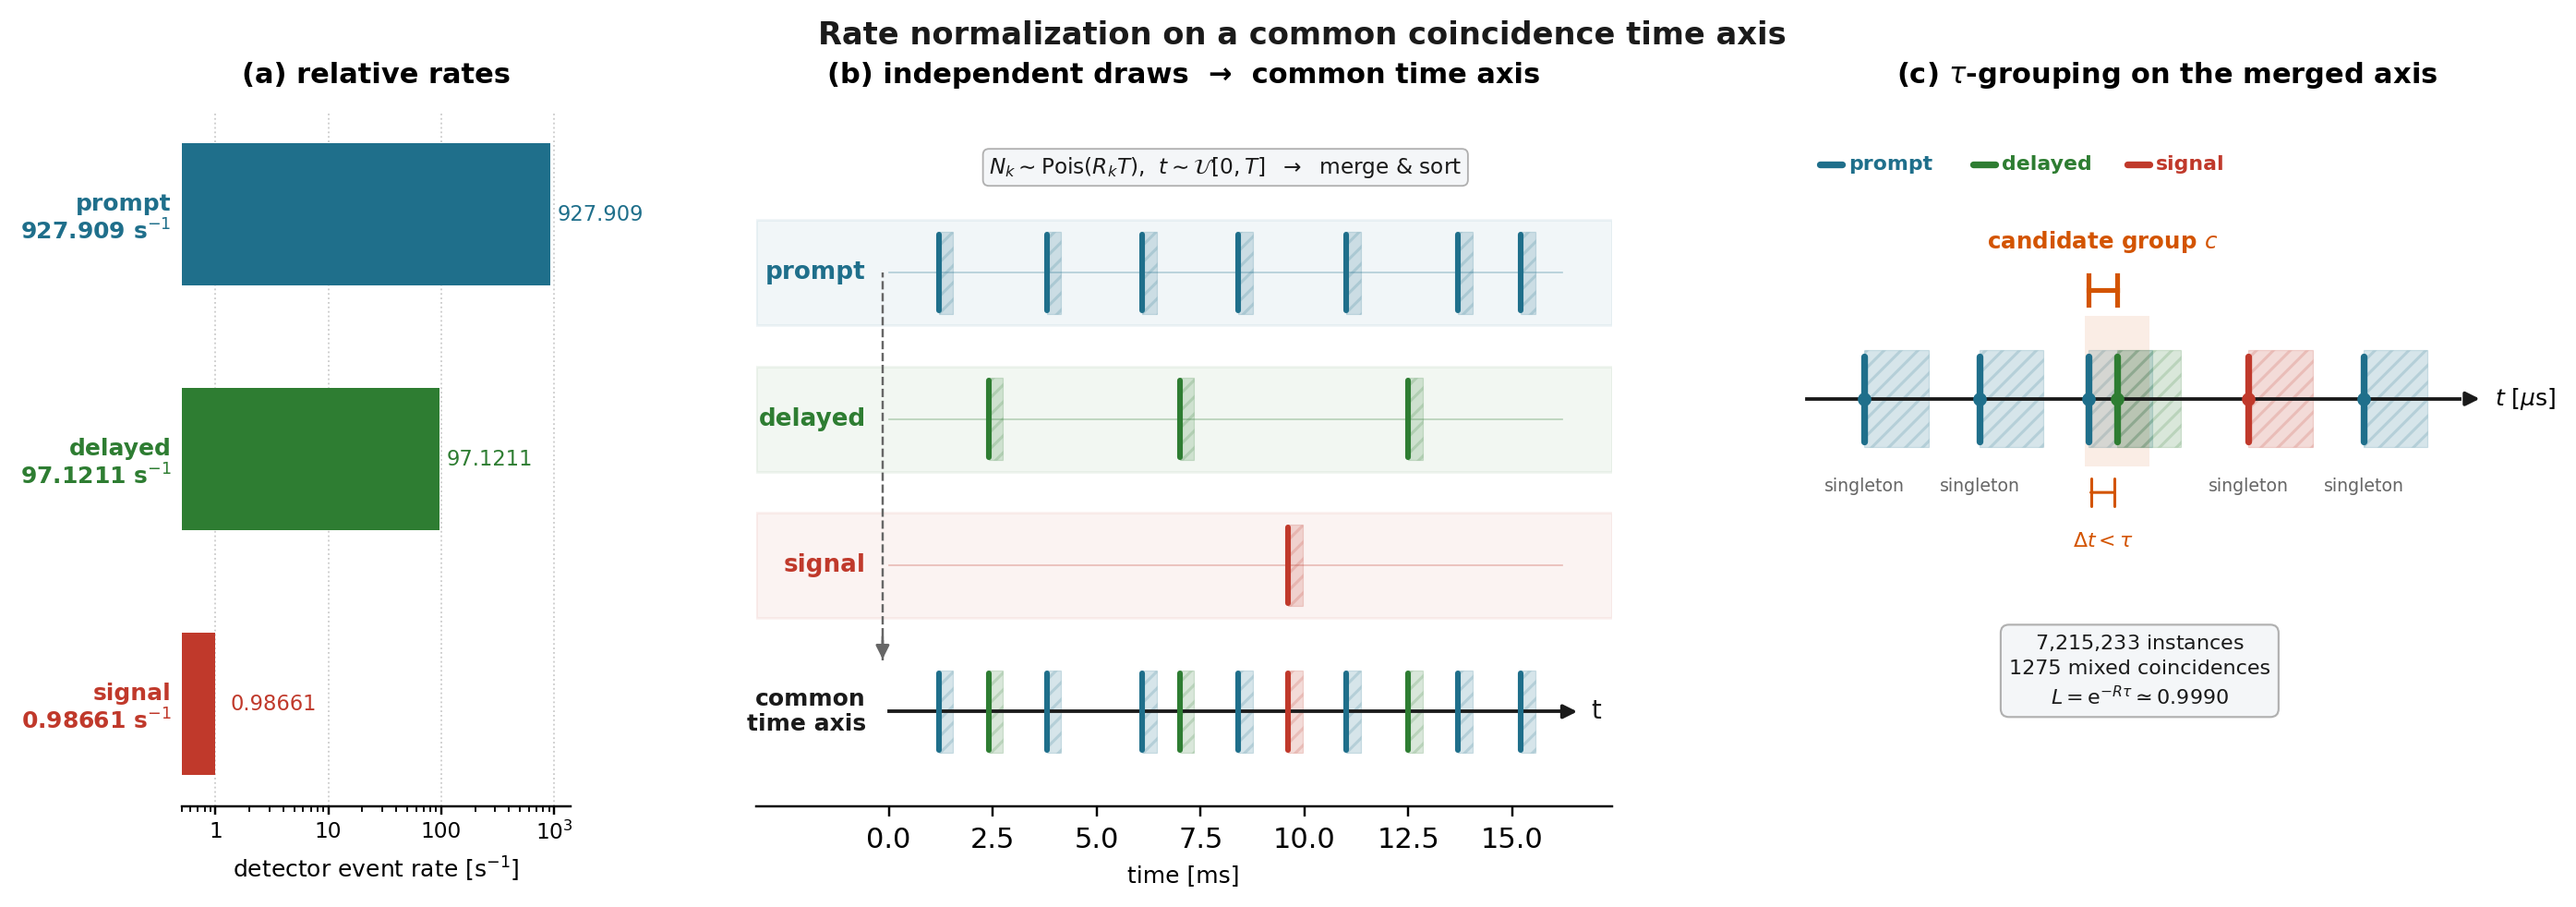
\includegraphics[width=\linewidth]{paper_source_figure_table/fig_s33_poisson_normalization.png}
\caption{三流参考率归一与公共符合时间轴检验。(a)~全能段探测器事例率（$928$、$97.1$、$0.987\,\mathrm{s^{-1}}$）。(b)~三条流独立泊松抽样后合并排序到公共时间轴；颜色标识流身份，影线表示各事例的时间足迹。(c)~$\Delta t\le\tau=1\,\mu\mathrm{s}$ 的事例归为一个符合候选组；框内为参考曝光的偶然符合计数。事例位置为示意。最终任务折叠另通过式~\eqref{eq:atm511_live_factor_zh} 纳入大气线占有率。}
\label{fig:s33_poisson}
\end{figure}

\begin{figure}[t]
\centering
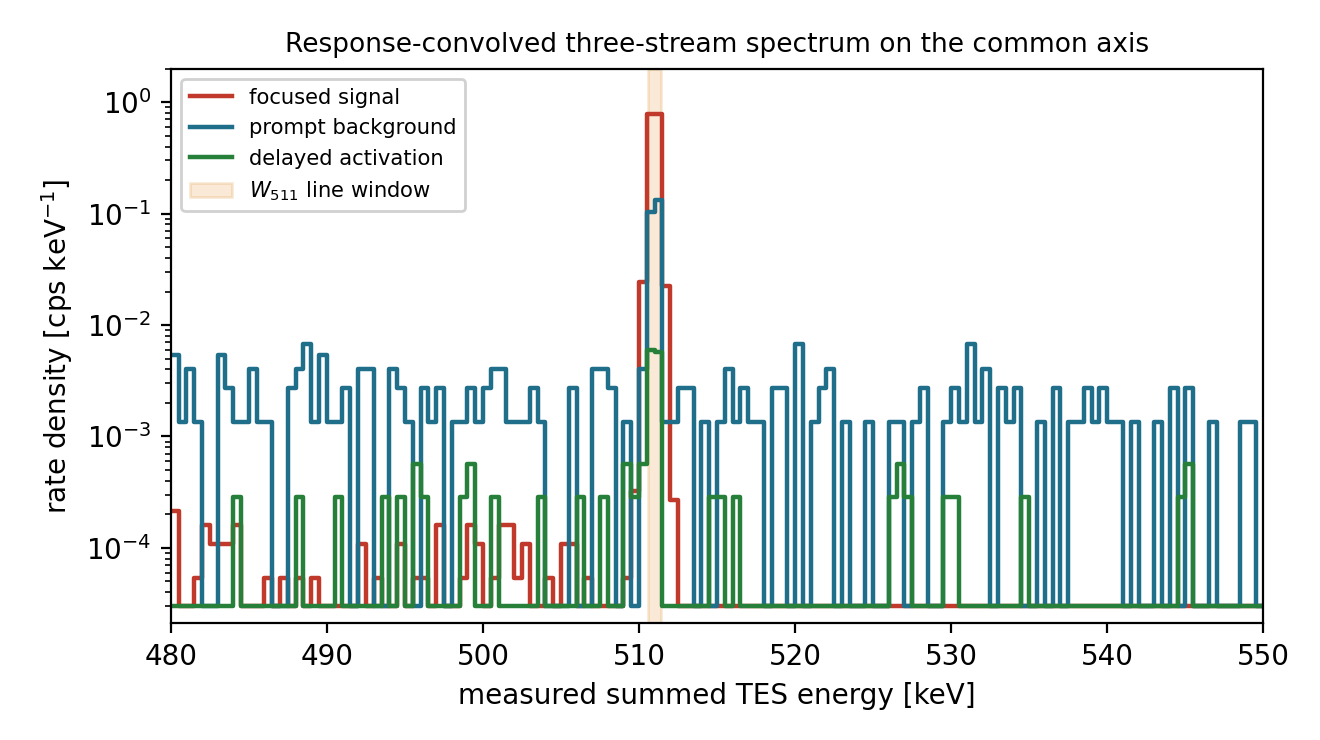
\includegraphics[width=0.72\linewidth]{paper_source_figure_table/fig_s33_spectrum_normalized.png}
\caption{三个参考分量在 veto 前公共时间轴上的响应卷积求和能谱。聚焦信号、瞬发与延迟分量均集中于 511 keV 线，连续谱计数较少。主线窗绝对选后率见表~\ref{tab:phase2_cutflow}。}
\label{fig:s33_spec_norm}
\end{figure}

图~\ref{fig:s33_poisson} 和图~\ref{fig:s33_spec_norm} 的显式泊松实现仅用于参考检验，不含大气线事例目录。最终轨迹计算分别推进大气线选后率，并在时间箱 $\ell$ 的活时间因子中加入其探测器占有率：
\begin{equation}
  L_{\ell}=\exp\!\left\{-\tau\left[
  R^{\mathrm{occ}}_{\mathrm{prompt},\ell}+
  R^{\mathrm{occ}}_{\mathrm{delayed},\ell}+
  R^{\mathrm{occ}}_{\mathrm{atm511},\ell}\right]\right\}.
  \label{eq:atm511_live_factor_zh}
\end{equation}
在大气线源的第 15 天参考状态，事例目录中有 $1{,}041{,}505$ 条事例至少包含一个 TES
或主动屏蔽命中，对应
$R^{\mathrm{occ}}_{\mathrm{atm511}}(15)=202.477\,\mathrm{s^{-1}}$。参考源流量下的
聚焦全能段率为 $0.987\,\mathrm{s^{-1}}$，故
$R^{\mathrm{occ}}_{\mathrm{sig}}\tau\simeq9.9\times10^{-7}$；本文在弱源近似下忽略
信号自符合。推广到更亮源时，应在指数中加入
$R^{\mathrm{occ}}_{\mathrm{sig},\ell}$。
主动反符合门在同一 $\tau$ 窗内比较 TES 与主动屏蔽沉积，拓扑重建则判断哪些命中属于同一入射光子。所有输运分量采用相同的符合窗和屏蔽阈值。每个轨迹时间箱内的率视为平稳：大气柱密度与活化库存按任务日尺度演化，而符合计算对应微秒至秒尺度。独立常率到达过程因而可按齐次泊松过程叠加。任务折叠使用各率的期望值，不在每个时间箱重新引入一次随机实现；显式三流实现只检验符合分组和偶然符合计数。

\subsubsection{主动反符合门}

第一层为统一时间轴上的主动反符合门。对每个符合候选组 $c$，记其 TES 与主动屏蔽的能量和
\begin{equation}
  E_{\mathrm{TES}}^{(c)}=\sum_{j\in c}E_{\mathrm{TES},j},\qquad
  E_{\mathrm{sh}}^{(c)}=\sum_{j\in c}E_{\mathrm{sh},j}.
\end{equation}
若 $E_{\mathrm{TES}}^{(c)}$ 落入分析线窗
\begin{equation}
  \wii = [510.58,511.42]\keV \quad (511\keV\pm420\,\mathrm{eV}),
\end{equation}
其为主要参考线窗，在保留主要线响应的同时抑制连续谱本底。若同时满足
\begin{equation}
  E_{\mathrm{sh}}^{(c)} < E_{\mathrm{veto}}, \qquad E_{\mathrm{veto}}=50\keV,
\end{equation}
则通过主动屏蔽，其中屏蔽能量在基准 CsI 配置下由 CsI 主动屏蔽体积于后处理读出。该层是率级本底压低的主要来源。逐像素施加探测器响应与阈值后，该门把瞬发本底从 $148$ 个事例（$0.1146\cps$）压到 $68$ 个（$0.04612\cps$，存活 $40.24\%$）、延迟活化从 $40$ 压到 $26$（存活 $65.00\%$），而聚焦信号 $28534$ 个事例全部保留（屏蔽零沉积，存活 $100\%$）；详见表~\ref{tab:phase2_cutflow}。其对背景能谱的作用见图~\ref{fig:s33_spec_anti}。

\begin{figure}[t]
\centering
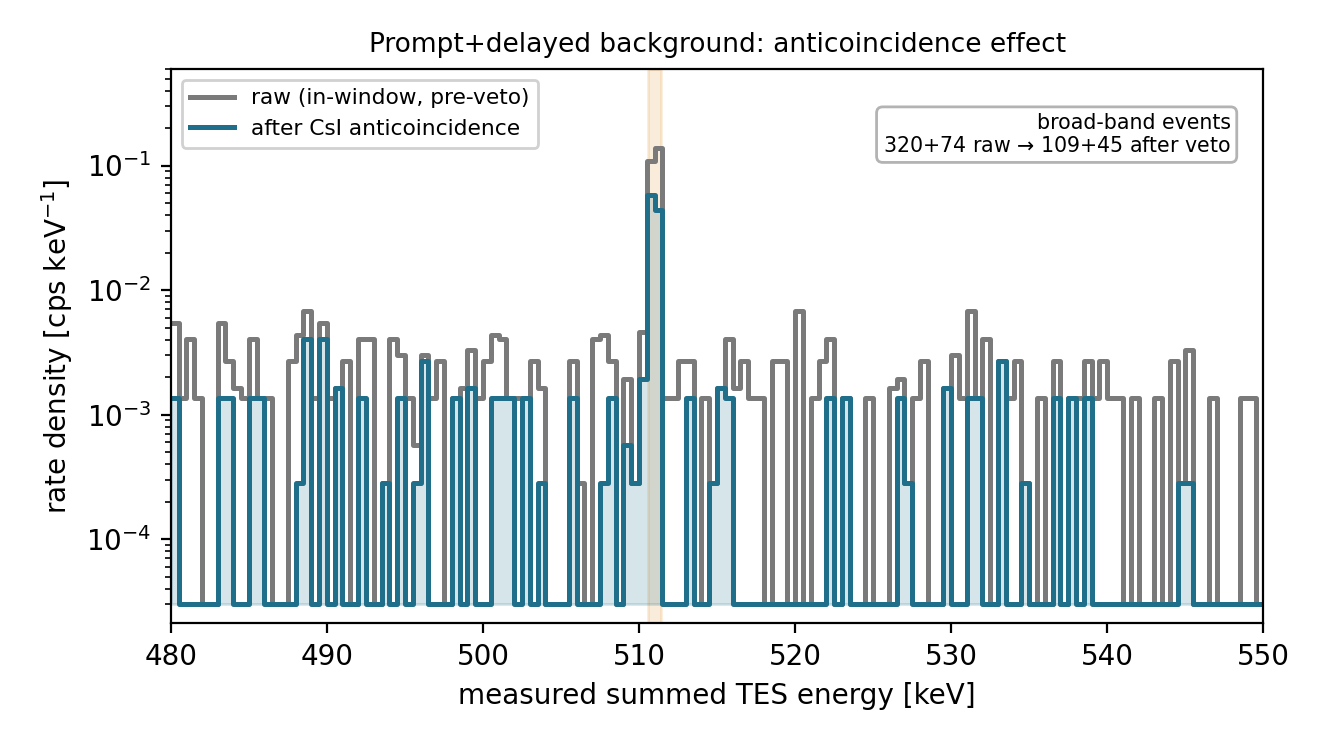
\includegraphics[width=0.72\linewidth]{paper_source_figure_table/fig_s33_spectrum_anticoincidence.png}
\caption{CsI 主动反符合门对瞬发$+$延迟背景能谱的作用（线窗内预 veto 对反符合后）。形状诊断，取自现存参考探测器事例目录的重导出。}
\label{fig:s33_spec_anti}
\end{figure}本文给出的流量阈值适用于经探测器响应后本征宽度相对该线窗仍较小的谱线；若源线明显展宽，须将源线型与响应卷积并重新优化窗宽。

\subsubsection{康普顿拓扑与视场一致性}

第二层对通过主动屏蔽的 TES 命中施加基于康普顿运动学的拓扑与视场一致性检验，其物理基础是康普顿相机的成锥重建~\cite{Zoglauer2006}。能量为 $E_0$ 的入射光子在第一作用点 $\mathbf r_1$ 发生康普顿散射、沉积能量 $E_1$，散射光子携带能量 $E_{\mathrm{sc}}=E_0-E_1$ 前进至下一作用点 $\mathbf r_2$，散射角 $\theta_C$ 由
\begin{equation}
  \cos\theta_C =
  1 - m_ec^2\left(\frac{1}{E_{\mathrm{sc}}}
  - \frac{1}{E_1+E_{\mathrm{sc}}}\right)
\end{equation}
给出。已知散射光子的飞行方向 $\hat{\mathbf u}_{12}=(\mathbf r_2-\mathbf r_1)/|\mathbf r_2-\mathbf r_1|$ 后，源的方位被约束在以 $\mathbf r_1$ 为顶点、$-\hat{\mathbf u}_{12}$ 为轴、半张角 $\theta_C$ 的重建圆锥面上，其在天球上的投影即事例圆。这里把第一散射锥用于孔径一致性检验：当锥面与侧入射 Be 窗圆盘（半径 $1.898\,\mathrm{cm}$）相交，即保留该事例，亦即其重建来向与穿过入射孔径相容。

由于单个 TES 像素（$1.5\times1.5\times3.0\,\mathrm{mm}$）的内部作用位置不可分辨，本文不以像素质心单点、而以 $8+1=9$ 个代表点（八个像素角点与质心）表征每个命中，从而把亚像素位置不确定性显式带入几何重建。据此，一个双命中事例在给定散射次序下枚举 $9\times9=81$ 组首/次作用点组合，对每组构造一条重建圆锥（锥面以 24 个方位角离散采样后延拓至 Be 窗平面，并同时以采样点与相邻线段判定与窗盘的相交）；只要这 81 条轨迹中存在任一条使锥面与 Be 窗盘相交，即判该次序视场相容。这是一个刻意从宽的一致性判据：只要像素内部存在与穿过入射孔径相容的作用位置假设即予保留。因此该层保留了约 $95\%$ 的窗内多命中事例、仅削减约 $10$--$14\%$ 的本底，与其宽松一致性 veto、而非成像重建的定位一致。

据此对三类事例分别处理。单像素事例无散射拓扑，直接作为量热线候选保留。双命中事例给出两点位置与能量，但缺少判定作用先后的内部信息，故对两种散射次序各枚举上述 81 条轨迹，只要任一次序视场相容即保留该事例，仅当两种次序均不存在运动学有效锥时判否。三命中及更高多重度事例含有内部散射顶点，可据几何—运动学一致性定序：在每个内部顶点上，散射角既可由能量经康普顿公式求得，又可由相邻两段飞行方向的夹角求得，二者对正确次序应当一致。本文枚举全部次序（至多六个 TES 命中，超出者不再定序而径直保留），以康普顿序列残差
\begin{equation}
  Q = \sum_{i=1}^{n-2}
  \left(\cos\theta_{C,i} -
  \hat{\mathbf u}_{i-1,i}\cdot\hat{\mathbf u}_{i,i+1}\right)^2
\end{equation}
取最小者为最优次序（残差并列时取首散射杠杆臂最长者），再对其首两点施加同一“81 轨迹—窗盘相交”检验。凡无任何有效次序者归为未重建类。在响应卷积后的基准中，通过主动屏蔽的事例经拓扑检验分为单点、视场相容的重建多点与否决三类：瞬发 $68=42$ 单点 $+\,21$ 重建多点 $+\,5$ 否决，延迟 $26=19+7+0$，聚焦信号 $28534=17267$ 单点 $+\,10726$ 重建多点 $+\,541$ 否决，故三流选后分别为 $63$、$26$、$27993$ 个事例。在 $480$--$550\,\keV$ 宽能带上，同一响应与选择把选后聚焦信号分解为 $17602$ 单点、$9793$ 双命中与 $2338$ 三命中及以上（其中 $370$ 双命中与 $262$ 三命中及以上被康普顿否决）；瞬发的对应选后多重度为 $62/27/6$，延迟为 $28/12/3$（图~\ref{fig:s33_compton_mult}）。

\begin{figure}[t]
\centering
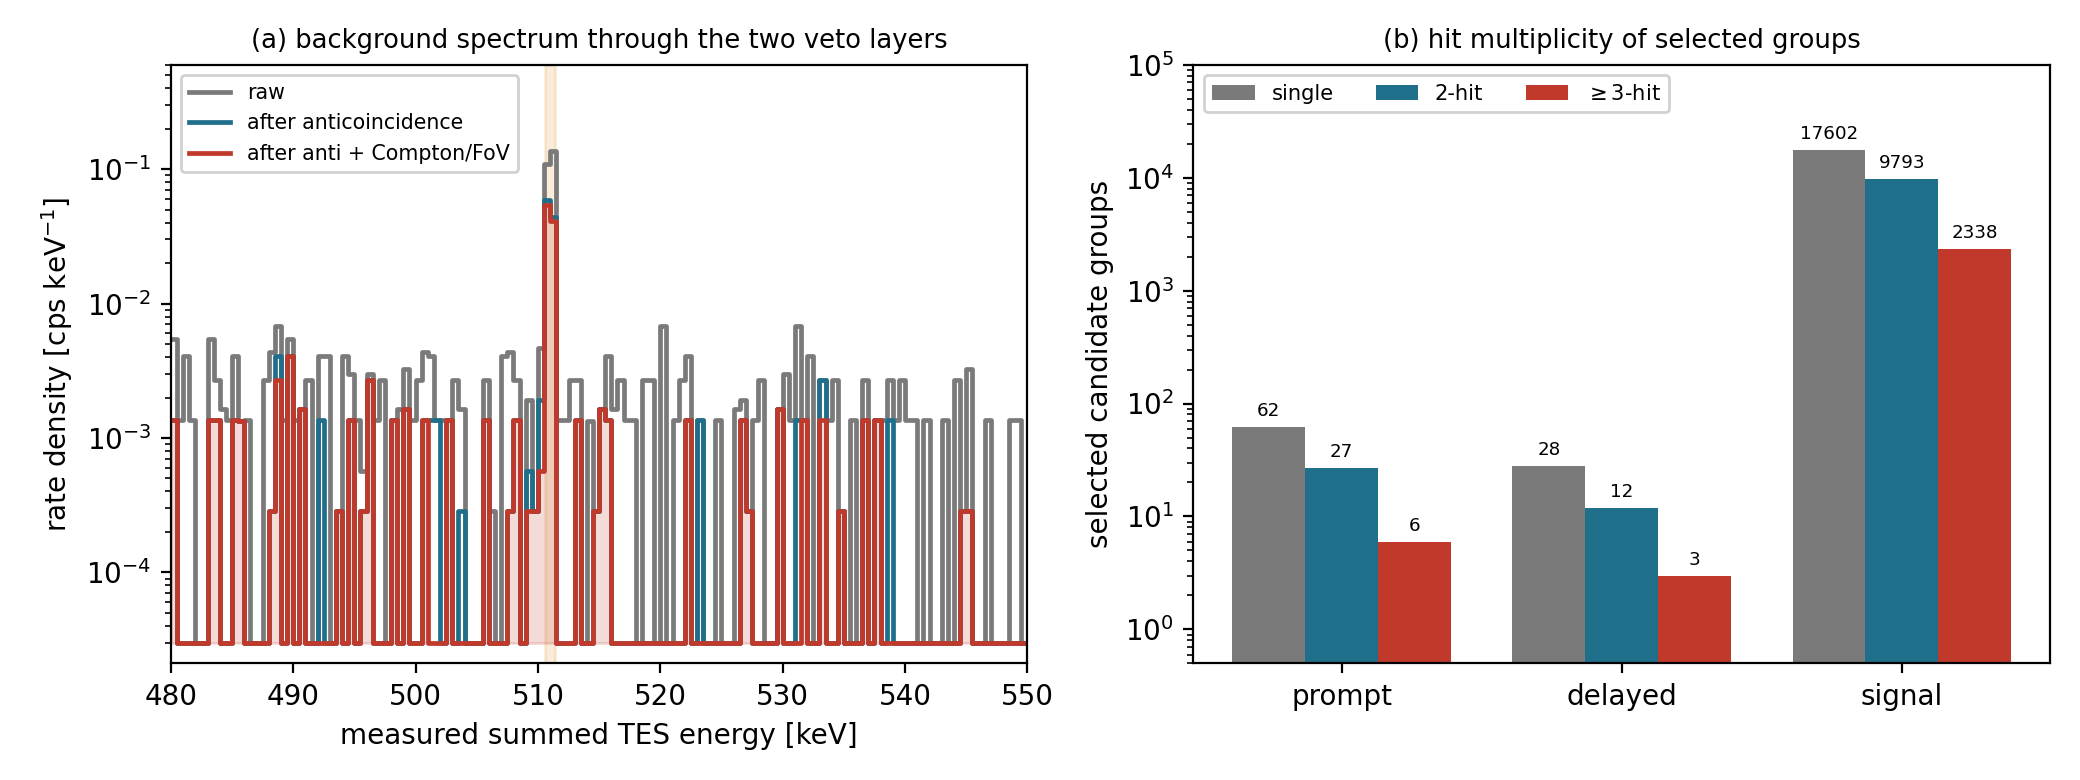
\includegraphics[width=\linewidth]{paper_source_figure_table/fig_s33_compton_multiplicity.png}
\caption{(a) 响应卷积后的背景能谱经两层 veto 的演化（raw；反符合后；反符合$+$康普顿/视场后）。(b) $480$--$550\,\keV$ 宽能带中各流选后候选组的 TES 命中多重度。主线窗绝对率见表~\ref{tab:phase2_cutflow}。}
\label{fig:s33_compton_mult}
\end{figure}

未重建类保留在基准率核算中，但不标记为视场通过候选。多命中接收的作用可直接量化：若仅保留单像素事例，在当前 $\wii$ 样本中将保留 $61.68\%$ 的聚焦信号率与 $67.17\%$ 的选后本底率，简单 $S/\sqrt{B}$ 降至基准值的 $0.753$。因此，本文采用的宽松多命中策略保留统计灵敏度，并把拓扑层用于一致性 veto，而非成像切选。

表~\ref{tab:phase2_cutflow} 用相同 TES 能窗、CsI veto 和康普顿/视场检验汇总参考几何的事例流。第一阶段是施加两层 veto 之前的线窗样本，统计不确定度由事例率权重的二次和给出。

\begin{table}[t]
\centering
\caption{参考几何的事例级 $\wii$ 线窗 cut-flow。聚焦信号率按单位 EventList 输入率归一；物理点源率另行缩放。}
\label{tab:phase2_cutflow}
\footnotesize
\resizebox{\linewidth}{!}{%
{
\begin{tabular}{llccc}
\toprule
流 & 阶段 & 事例数 & 率 / $\cps$ & 统计不确定度 / $\cps$ \\
\midrule
瞬发本底 & 线窗预 veto & 148 & $1.14624\times10^{-1}$ & $1.24549\times10^{-2}$ \\
瞬发本底 & CsI veto 后 & 68 & $4.61248\times10^{-2}$ & $5.59345\times10^{-3}$ \\
瞬发本底 & 拓扑/视场选后 & 63 & $4.27321\times10^{-2}$ & $5.38374\times10^{-3}$ \\
延迟活化 & 线窗预 veto & 40 & $5.69229\times10^{-3}$ & $9.00030\times10^{-4}$ \\
延迟活化 & CsI veto 后 & 26 & $3.69999\times10^{-3}$ & $7.25627\times10^{-4}$ \\
延迟活化 & 拓扑/视场选后 & 26 & $3.69999\times10^{-3}$ & $7.25627\times10^{-4}$ \\
聚焦信号 & 线窗预 veto & 28534 & $7.67167\times10^{-1}$ & $4.54160\times10^{-3}$ \\
聚焦信号 & CsI veto 后 & 28534 & $7.67167\times10^{-1}$ & $4.54160\times10^{-3}$ \\
聚焦信号 & 拓扑/视场选后 & 27993 & $7.52621\times10^{-1}$ & $4.49834\times10^{-3}$ \\
\bottomrule
\end{tabular}
}}
\vspace{0.5ex}
\begin{minipage}{0.94\linewidth}
\footnotesize
聚焦信号行给出单位 EventList 输入率下的传输率，用于展示各选择步骤的保留比例；点源的物理信号率另按 Laue 有效面积、参考通量和大气透过率缩放。
\end{minipage}
\end{table}

本文另用 MEGAlib \texttt{revan} 康普顿事例重建器对保留旧几何中的 $37{,}065$ 个聚焦信号事例建立独立拓扑基准~\cite{Zoglauer2006}。该样本不与上述响应卷积后的参考探测器率预算混合，而用于检验作用次序与角分辨诊断。就双命中定序而言，基准给出两条定量结论：其一，“至少存在一个运动学有效次序”的比例为 $100.0\%$（$10{,}421/10{,}421$），与解析预期一致——全吸收 $511\keV$ 的双命中，其散射光子能量不低于康普顿边对应的 $E_0/3$，故必有一序满足——保留双命中事例的前提由此成立；其二，由 Klein--Nishina 截面加运动学品质因子选出的最优次序仅有 $78.4\%$ 与更指向源方向的次序一致，故若如成像链般只承诺单一估计次序，约 $22\%$ 的双命中事例将采用错误的康普顿锥，而枚举两个次序并取其一与视场相容则规避了这一错配。窗内康普顿事例相对真实束方向的 $|\mathrm{ARM}|$ 中位数约为 $24^\circ$（双命中 $23.6^\circ$、三命中及以上 $26.3^\circ$；$|\mathrm{ARM}|<10^\circ$ 者仅约 $32\%$），其根源是毫米量级的散射杠杆臂与像素量化；这从物理上解释了拓扑/视场层为何仅削减约 $10$--$14\%$ 的本底、且无法升级为成像级判别。不可定序事例的占比极小（\texttt{revan} 侧 $61/37{,}065$，即 $0.16\%$；解析分类器侧仅 $1$ 个），表明未重建类是一个很小的边界类。

\subsection{任务时间轨迹与解析率折叠}
\label{sec:mission_time_fold}

MeV 波段气球观测本质上是本底主导的：大气次级粒子与宇宙线诱发的仪器活化共同设定率底，且二者都对飞行环境敏感 \cite{Gallego2025Balloon,Kierans2017}。在固定质量模型下，探测器耦合 Monte Carlo 已给出第 15 天参考状态下、经统一 veto 与能窗的选后信号与本底率（第~\ref{sec:background}--\ref{sec:selection}~节）。但这些率对应于单一经纬与海拔。在长达数日的浮空过程中，残余大气深度、地磁截止刚度与活化库存会随状态演化，因此不能把第 15 天快照按时间线性拉伸来代表整段飞行。与其他气球 MeV 计划类似（例如 COSI 沿飞行轨迹用 PARMA/EXPACS 场并引入时间依赖光变曲线 \cite{Gallego2025Balloon}），本文引入解析的任务时间--轨迹曲线，将参考率映射为连续 20\,d 性能估计，并用选定轨迹状态上的直接 Cosima 输运检验该折叠，而不是在每个时间箱重跑全统计量。

此处轨迹是\emph{合成参考剖面}，既非气球遥测，也非源可见性/指向时间表。它包含从第 0 天到第 20 天的 81 个时间箱（间隔 0.25\,d），并取温和的中纬度浮空包络：海拔 $h=38.75\pm2.5$\,km，纬度 $34^\circ\pm0.25^\circ$，经度 $100^\circ\pm0.25^\circ$，相位以第 15 天为锚。保留海拔起伏，是因为零压类及相近长航时气球在浮空段会出现高度变化，使残余大气深度改变若干 $\mathrm{g\,cm^{-2}}$；深度同时调制驱动瞬发本底与活化的大气粒子谱，以及乘在聚焦科学率上的 511\,keV 大气透过率。经纬度仅作为同一合成轨迹上对截止刚度的\emph{参考}地磁/地理调制，并不编码地球遮挡、目标仰角限制或转向损失。因而该折叠支撑的是受控轨迹包络下的\emph{参考曝光统计灵敏度}，而非某一具体发射航次的飞行预报。

解析折叠包含六个物理上彼此分离的层。大气透过率只乘在天体信号上，不重标驱动瞬发本底与活化的本地粒子场，也不重标式~\eqref{eq:atm511_flux_zh} 定义的大气线源。

\emph{（1）信号。}对大气层上单色点源流量 $F_{511}$，
\begin{equation}
  R_{\mathrm{sig}}(t)=F_{511}\,A_{\mathrm{eff}}\,T_{\mathrm{atm},511}(t)\,\varepsilon_{\mathrm{det}},
  \label{eq:mission_signal_zh}
\end{equation}
其中 $A_{\mathrm{eff}}$ 为轴上 Laue 有效面积，$T_{\mathrm{atm},511}(t)$ 为轨迹状态下 511\,keV 大气透过率，$\varepsilon_{\mathrm{det}}$ 归并参考响应下的探测器与选择效率。相对第 15 天锚点，等价于
$S_{\mathrm{sig}}(t)=S_{15}\,T_{\mathrm{atm},511}(t)/T_{15,45}$，且
$T_{15,45}=0.6520$。每个时间箱均采用固定 $45^\circ$ 仰角（天顶角亦为 $45^\circ$），
$T_{\mathrm{atm},511}(t)=\exp[-\mu_{\mathrm{air}}X_{\mathrm{vertical}}(t)/\cos45^\circ]$，
其中 $\mu_{\mathrm{air}}=0.08736\,\mathrm{cm^2\,g^{-1}}$。该式采用沿仪器光轴的斜程柱深，仍是固定光轴参考，而非源可见性计算。

\emph{（2）瞬发本底。}在粒子族分辨下，选后瞬发率为源--响应求和
\begin{equation}
  R_{\mathrm{prompt},j}(t)=\sum_{b}\Phi_{b}(t)\,K_{j,b},
  \label{eq:prompt_source_response_zh}
\end{equation}
其中 $b$ 遍历大气粒子族（质子、中子、$e^{\pm}$、$\gamma$、$\mu^{\pm}$ 等），$\Phi_{b}(t)$ 为在对应轨迹状态重新计算的 PARMA/EXPACS 通量，$K_{j,b}$ 是在第 15 天参考输运上为选择 $j$ 固定一次的探测器响应系数。相对参考态，这等价于按 $\Phi_{b}(t)/\Phi_{b}(\mathrm{REF})$ 重加权各族贡献。在线窗内，若具备能量--角度响应矩阵，可将同一结构细化为 $K_{b,E,\theta}$。

\emph{（3）大气 511 keV 线。}独立输运的第 15 天大气线响应按全空间线积分通量缩放：
\begin{equation}
  R_{\mathrm{atm511},j}(t)=R_{\mathrm{atm511},j}(15)
  \frac{\Phi_{4\pi}(t)}{\Phi_{4\pi}(15)},\qquad
  R^{\mathrm{occ}}_{\mathrm{atm511}}(t)=R^{\mathrm{occ}}_{\mathrm{atm511}}(15)
  \frac{\Phi_{4\pi}(t)}{\Phi_{4\pi}(15)}.
  \label{eq:mission_atm511_zh}
\end{equation}
其中 $\Phi_{4\pi}(t)$ 由式~\eqref{eq:atm511_flux_zh} 沿大气线代理深度与刚度曲线计算，
该曲线第 15 天取 $11.0\,\mathrm{GV}$；它不同于第 15 天取 $11.6\,\mathrm{GV}$ 的状态相关
PARMA 瞬发场。任务折叠改变总线通量，但固定已输运的第 15 天角响应；大气线不在每个
时间箱重新输运。

\emph{（4）活化产生。}对最终全八族延迟清单中的每个入射族 $a$ 与放射性源母核素 $k$，
\begin{equation}
  P_{a,k}(t)=\Phi_{a}(t)\,Y_{a,k},
  \label{eq:activation_production_zh}
\end{equation}
其中 $Y_{a,k}$ 是由对应第 15 天清单固定的分族产额，$\Phi_a(t)$ 是该族在各轨迹状态
重新计算的 PARMA 通量。质量完备参考几何的 $141.83\,\mathrm{Bq}$ 全粒子族清单用于
本底来源分析，不替代这条最终几何任务折叠；后者使用最终方向分级构型的
$36.4525153\,\mathrm{Bq}$ 清单。

\emph{（5）延迟库存。}设衰变常数 $\lambda_k$，每个“入射族--源母核素”库存按
\begin{equation}
  N_{a,k}(t+\Delta t)=N_{a,k}(t)\,e^{-\lambda_k\Delta t}
  +\frac{P_{a,k}(t)}{\lambda_k}\bigl(1-e^{-\lambda_k\Delta t}\bigr),
  \qquad A_{a,k}(t)=\lambda_k N_{a,k}(t)
  \label{eq:delayed_inventory_zh}
\end{equation}
推进。

\emph{（6）延迟选后率。}
\begin{equation}
  R_{\mathrm{delayed},j}(t)=\sum_{a}\sum_{k} A_{a,k}(t)\,\varepsilon_{j,a,k},
  \label{eq:delayed_selected_zh}
\end{equation}
其中 $\varepsilon_{j,a,k}$ 为入射族 $a$ 产生的源母核素 $k$ 在选择 $j$ 下的选后率响应。SIM 的 IA INIT 女核身份保留为谱系证据，但不替代该求和中的放射性源母核。式~\eqref{eq:mission_signal_zh}--\eqref{eq:delayed_selected_zh} 将天体信号透过、瞬发粒子调制、大气线缩放、活化产生与放射性衰变保持为相互独立的物理步骤。

为检验解析预测，选取并固定四个轨迹状态——第 15 天参考（REF）、低空早期点（L1）、
高空点（H1）与低空晚期点（L2）——并在这些坐标上重新计算 PARMA 谱与 Cosima
大气源，\emph{不}把解析尺度当作自由参数。对式~\eqref{eq:prompt_source_response_zh}
给出的预测尺度 $S^{\mathrm{pred}}$ 定义
\begin{equation}
  Q=\frac{R^{\mathrm{MC}}/R^{\mathrm{MC}}_{\mathrm{REF}}}{S^{\mathrm{pred}}}.
\end{equation}
理想一致时 $Q\simeq1$。最终实现分别用各轨迹状态的 PARMA 通量比缩放八类瞬发粒子
各自的第 15 天响应系数，并用各自匹配的族通量比推进每个保留的“族--母核素”延迟
分量。在 TES 宽能带 $480$--$550$\,keV 上，直接轨迹输运对合并 $e^+$、$n$ 与
$\gamma$ 调制的检验在 $2\sigma$ 内一致（偏离参考点的最大 $|z|\simeq0.51$）；仅取
高统计 $e^+$ 带时，$Q$ 相对重新计算的 PARMA $e^+$ 通量尺度维持在约 $1\%$ 内。
这些多点结果为已检验粒子族提供直接验证，其余瞬发粒子族仍采用解析源场重加权；所有
最终 511 keV 窄窗响应系数均由第 15 天完整探测器链给出。

在完整探测器链固定最终几何的第 15 天选后率之后，这些轨迹尺度给出式~\eqref{eq:cumulative_counts_zh} 中的 $S(t)$、$B(t)$ 与累计计数。第~\ref{sec:results}~节把中心显著度曲线和条件式逐分量输运计数端点画在同一时间轴上，使期望任务性能和有限输运 Monte Carlo 支撑的影响能够直接比较。

\section{结果}
\label{sec:results}

\subsection{511 keV 线窗本底由什么决定？}
\label{subsec:reference_background_results_zh}

质量完备参考几何先回答屏蔽设计之前的物理问题：究竟哪些相互作用进入科学能窗？在主 $510.58$--$511.42\keV$ 线窗中，经统一响应、主动 veto 与拓扑/视场选择后，保留 63 条瞬发和 26 条延迟 Monte Carlo 记录。由于各流代表的物理曝光不同，其事例权重也不同；这些记录对应的瞬发加延迟诊断率为 $(4.64320\pm0.54324)\times10^{-2}\cps$。表~\ref{tab:reference_background_budget_zh} 同时给出记录数和带权率；单独输运的大气 511\,keV 线不计入这一参考几何诊断。

\begin{table}[t]
\centering
\caption{参考探测器主线窗的瞬发加延迟诊断；单独输运的大气 511\,keV 线不在其中。相对不确定度为 Monte Carlo 计数标准误差。各分量独立归一，故记录数不与率贡献成正比。}
\label{tab:reference_background_budget_zh}
\footnotesize
\resizebox{\linewidth}{!}{%
\begin{tabular}{lrrrrrl}
\toprule
分量 & 选后记录 & 率 / $\cps$ & MC $\sigma$ / $\cps$ & 相对 MC $\sigma$ / \% & 总率占比 / \% & 选后事例来源 \\
\midrule
瞬发 $e^+$ & 43 & $2.91730\times10^{-2}$ & $4.44885\times10^{-3}$ & 15.2 & 62.83 & 入射粒子族标签 \\
瞬发 $n$ & 18 & $1.22099\times10^{-2}$ & $2.87791\times10^{-3}$ & 23.6 & 26.30 & 入射粒子族标签 \\
瞬发 $\mu^+$ & 2 & $1.34910\times10^{-3}$ & $9.53958\times10^{-4}$ & 70.7 & 2.91 & 入射粒子族标签 \\
瞬发小计 & 63 & $4.27321\times10^{-2}$ & $5.38374\times10^{-3}$ & 12.6 & 92.03 & 八类粒子输运 \\
延迟活化 & 26 & $3.69999\times10^{-3}$ & $7.25627\times10^{-4}$ & 19.6 & 7.97 & 24 条 $^{64}$Cu、2 条 $^{61}$Cu \\
\midrule
总计 & 89 & $4.64320\times10^{-2}$ & $5.43242\times10^{-3}$ & 11.7 & 100.00 & 瞬发加延迟 \\
\bottomrule
\end{tabular}}
\end{table}

\begin{figure}[t]
\centering
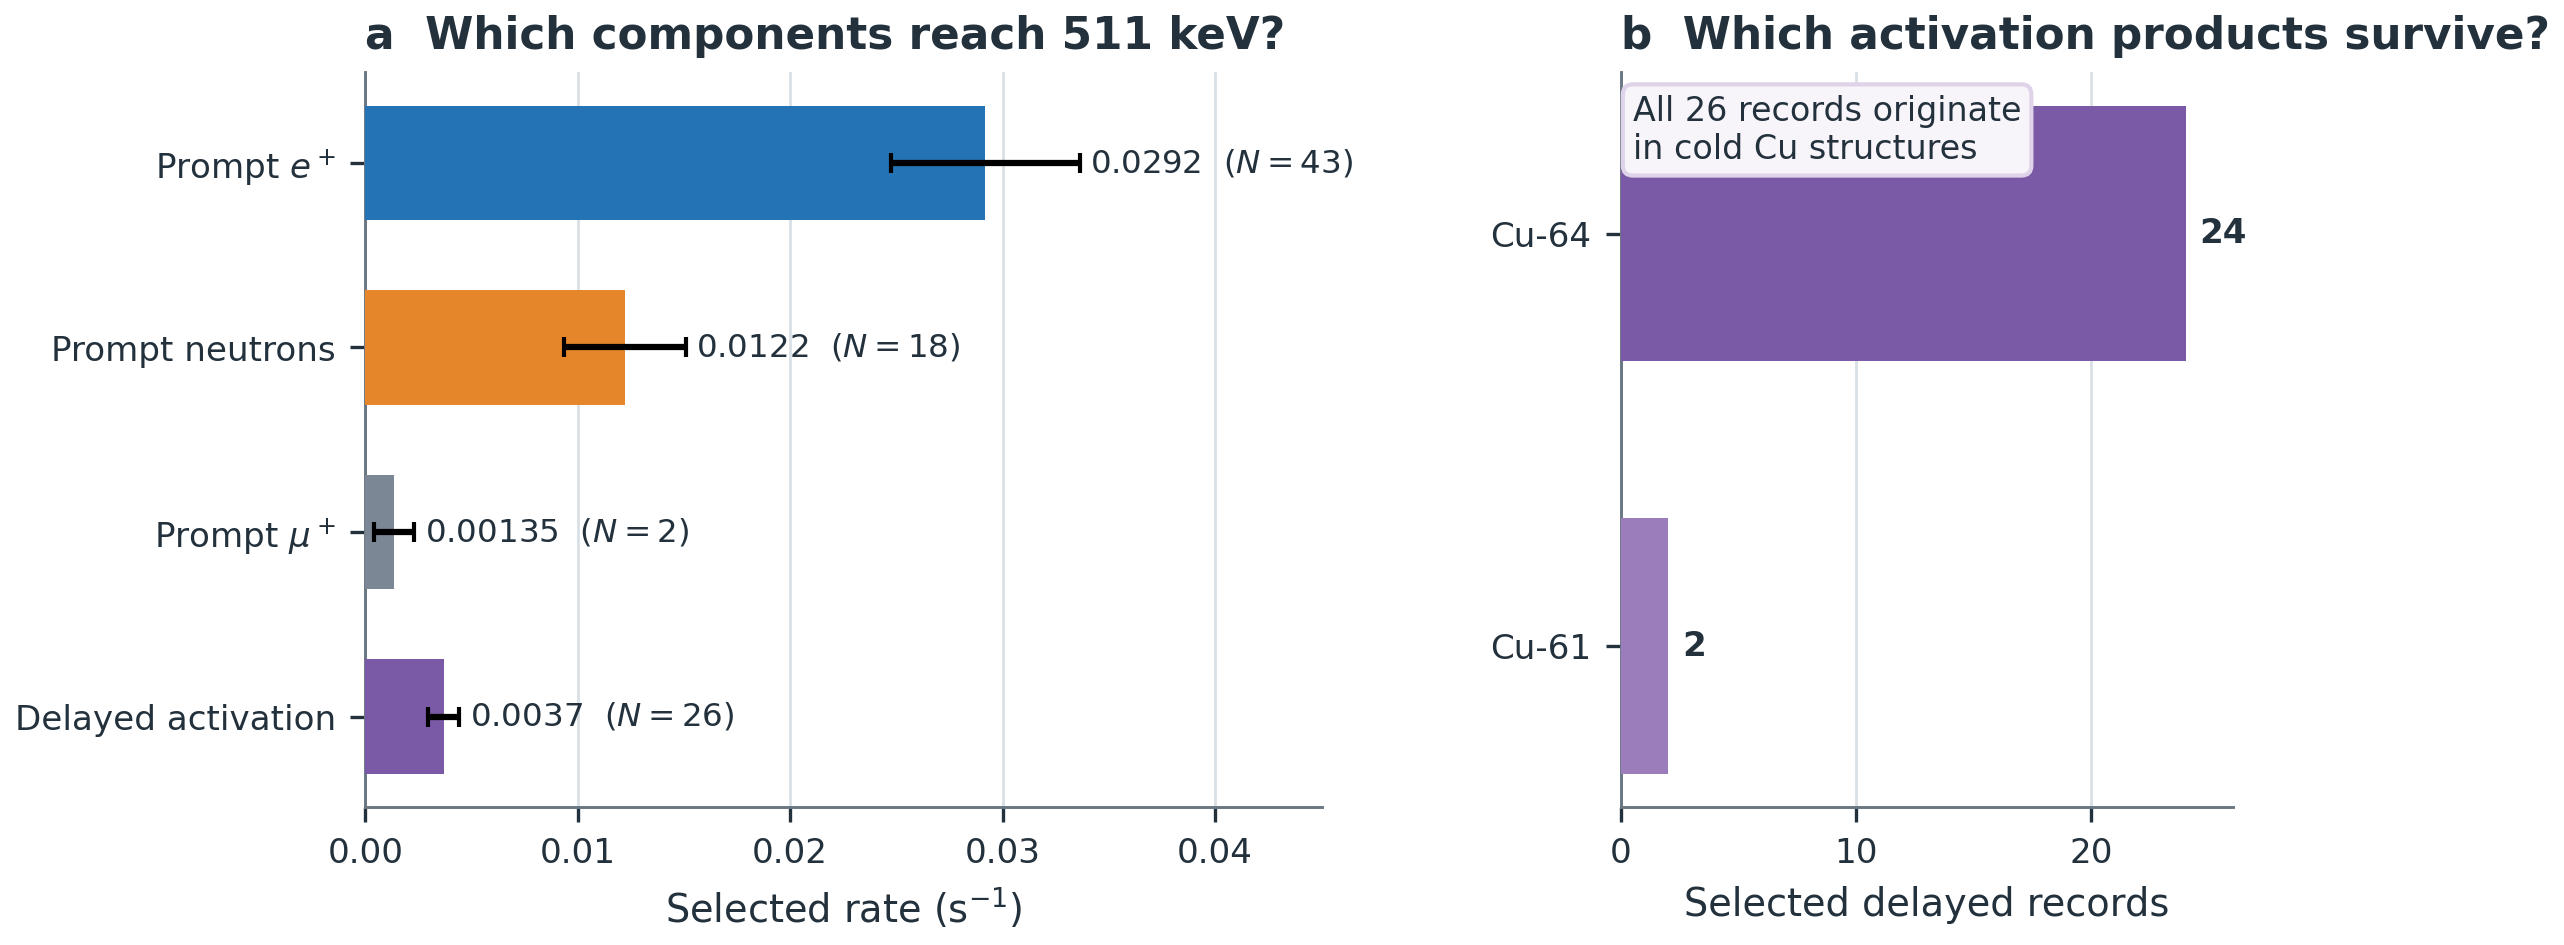
\includegraphics[width=0.98\linewidth]{paper_source_figure_table/fig_background_origin_story.png}
\caption{质量完备参考几何中选后瞬发加延迟诊断本底的物理来源；图中不含大气 511\,keV 线。（a）瞬发粒子族与延迟活化的带权率；误差棒为式~\eqref{eq:weighted_rate_stats_zh} 的 Monte Carlo 计数标准误差。（b）26 条选后延迟记录的母核素。正电子和中子合计贡献该诊断率的 $89.13\%$；全部延迟记录都产生于冷铜结构。}
\label{fig:background_origin_story_zh}
\end{figure}

图~\ref{fig:background_origin_story_zh} 给出瞬发结果。入射正电子贡献 $2.917\times10^{-2}\cps$，中子贡献 $1.221\times10^{-2}\cps$；二者合计占瞬发率的 $96.84\%$、占瞬发加延迟诊断率的 $89.13\%$。大气 511\,keV 线按第~\ref{subsec:atm511_source_zh}~小节的定义作为独立分量进入最终全链；在本文采用的探测器响应和线窗下，它与科学线在能谱上不可区分。全部八类瞬发粒子仍保留在最终输运中；这里的分解用于解释本底来源，而不是删去源类别。

延迟事例的源级分布与探测器选后分布不同。经修正的第 15 天总活度为
$141.83$ Bq，其中中子诱发产物占 $94.25\%$，$\mu^-$ 诱发产物占 $5.38\%$；
按材料分类后，CsI、外部机械结构和冷板分别占 $63.08\%$、$15.71\%$ 和
$9.43\%$，中子与 $\mu^-$ 的材料分布满足 $D_{\mathrm{TV}}=0.823$。经过探测器响应
和完整选择后，26 条线窗延迟记录中有 24 条来自冷铜结构中的 $^{64}$Cu，另 2 条来自
$^{61}$Cu。源清单和选后线窗本底因此给出不同的材料优先级：主动覆盖控制主导瞬发与
大气路径，焦平面附近的铜则提供局域延迟分量。

最终方向分级构型的活化结果来自另一套全八族计算。经 NUBASE 修正的第 15 天活度为 $36.4525153\,\mathrm{Bq}$：中子、$\mu^-$、质子和 $\alpha$ 分别贡献 $83.83\%$、$10.82\%$、$4.64\%$ 和 $0.69\%$，$e^+$、$\gamma$ 与 $\mu^+$ 还有更小的正活度清单；$e^-$ 为有限 BUILDUP 零观测。最终 78 条延迟记录由 60 条中子、12 条质子、5 条 $\mu^-$ 和 1 条 $\alpha$ 记录组成，任务折叠同时按入射族与精确位置源母核素分辨。特别地，唯一一条在 SIM 中从 $^{182}$W 开始的谱系归入位置匹配的放射性 $^{182}$Ta 源母核，而不是把稳定基态 $^{182}$W 当作活度。

\FloatBarrier

\subsection{最终方向分级主动屏蔽几何}
\label{subsec:optimized_shield_results_zh}

最终主动屏蔽把本底图转成一套简单结构。侧壁包围较长的低温系统外壳并包含光学侧孔，是最重要的主动表面，因此采用 40 mm BGO；底部采用 30 mm BGO 圆盘，顶部在服务开口周围采用 10 mm BGO 环。聚焦光束仍通过对准的侧孔进入。外部保留薄 Al/Kapton 包络，不设置连续外部 W 层。图~\ref{fig:optimized_shield_background_zh} 把这套结构连接到事例选择和最终本底预算，表~\ref{tab:final_geometry_zh} 给出尺寸；下文全链和任务计算只使用这一套优化几何。

\begin{figure}[!ht]
\centering
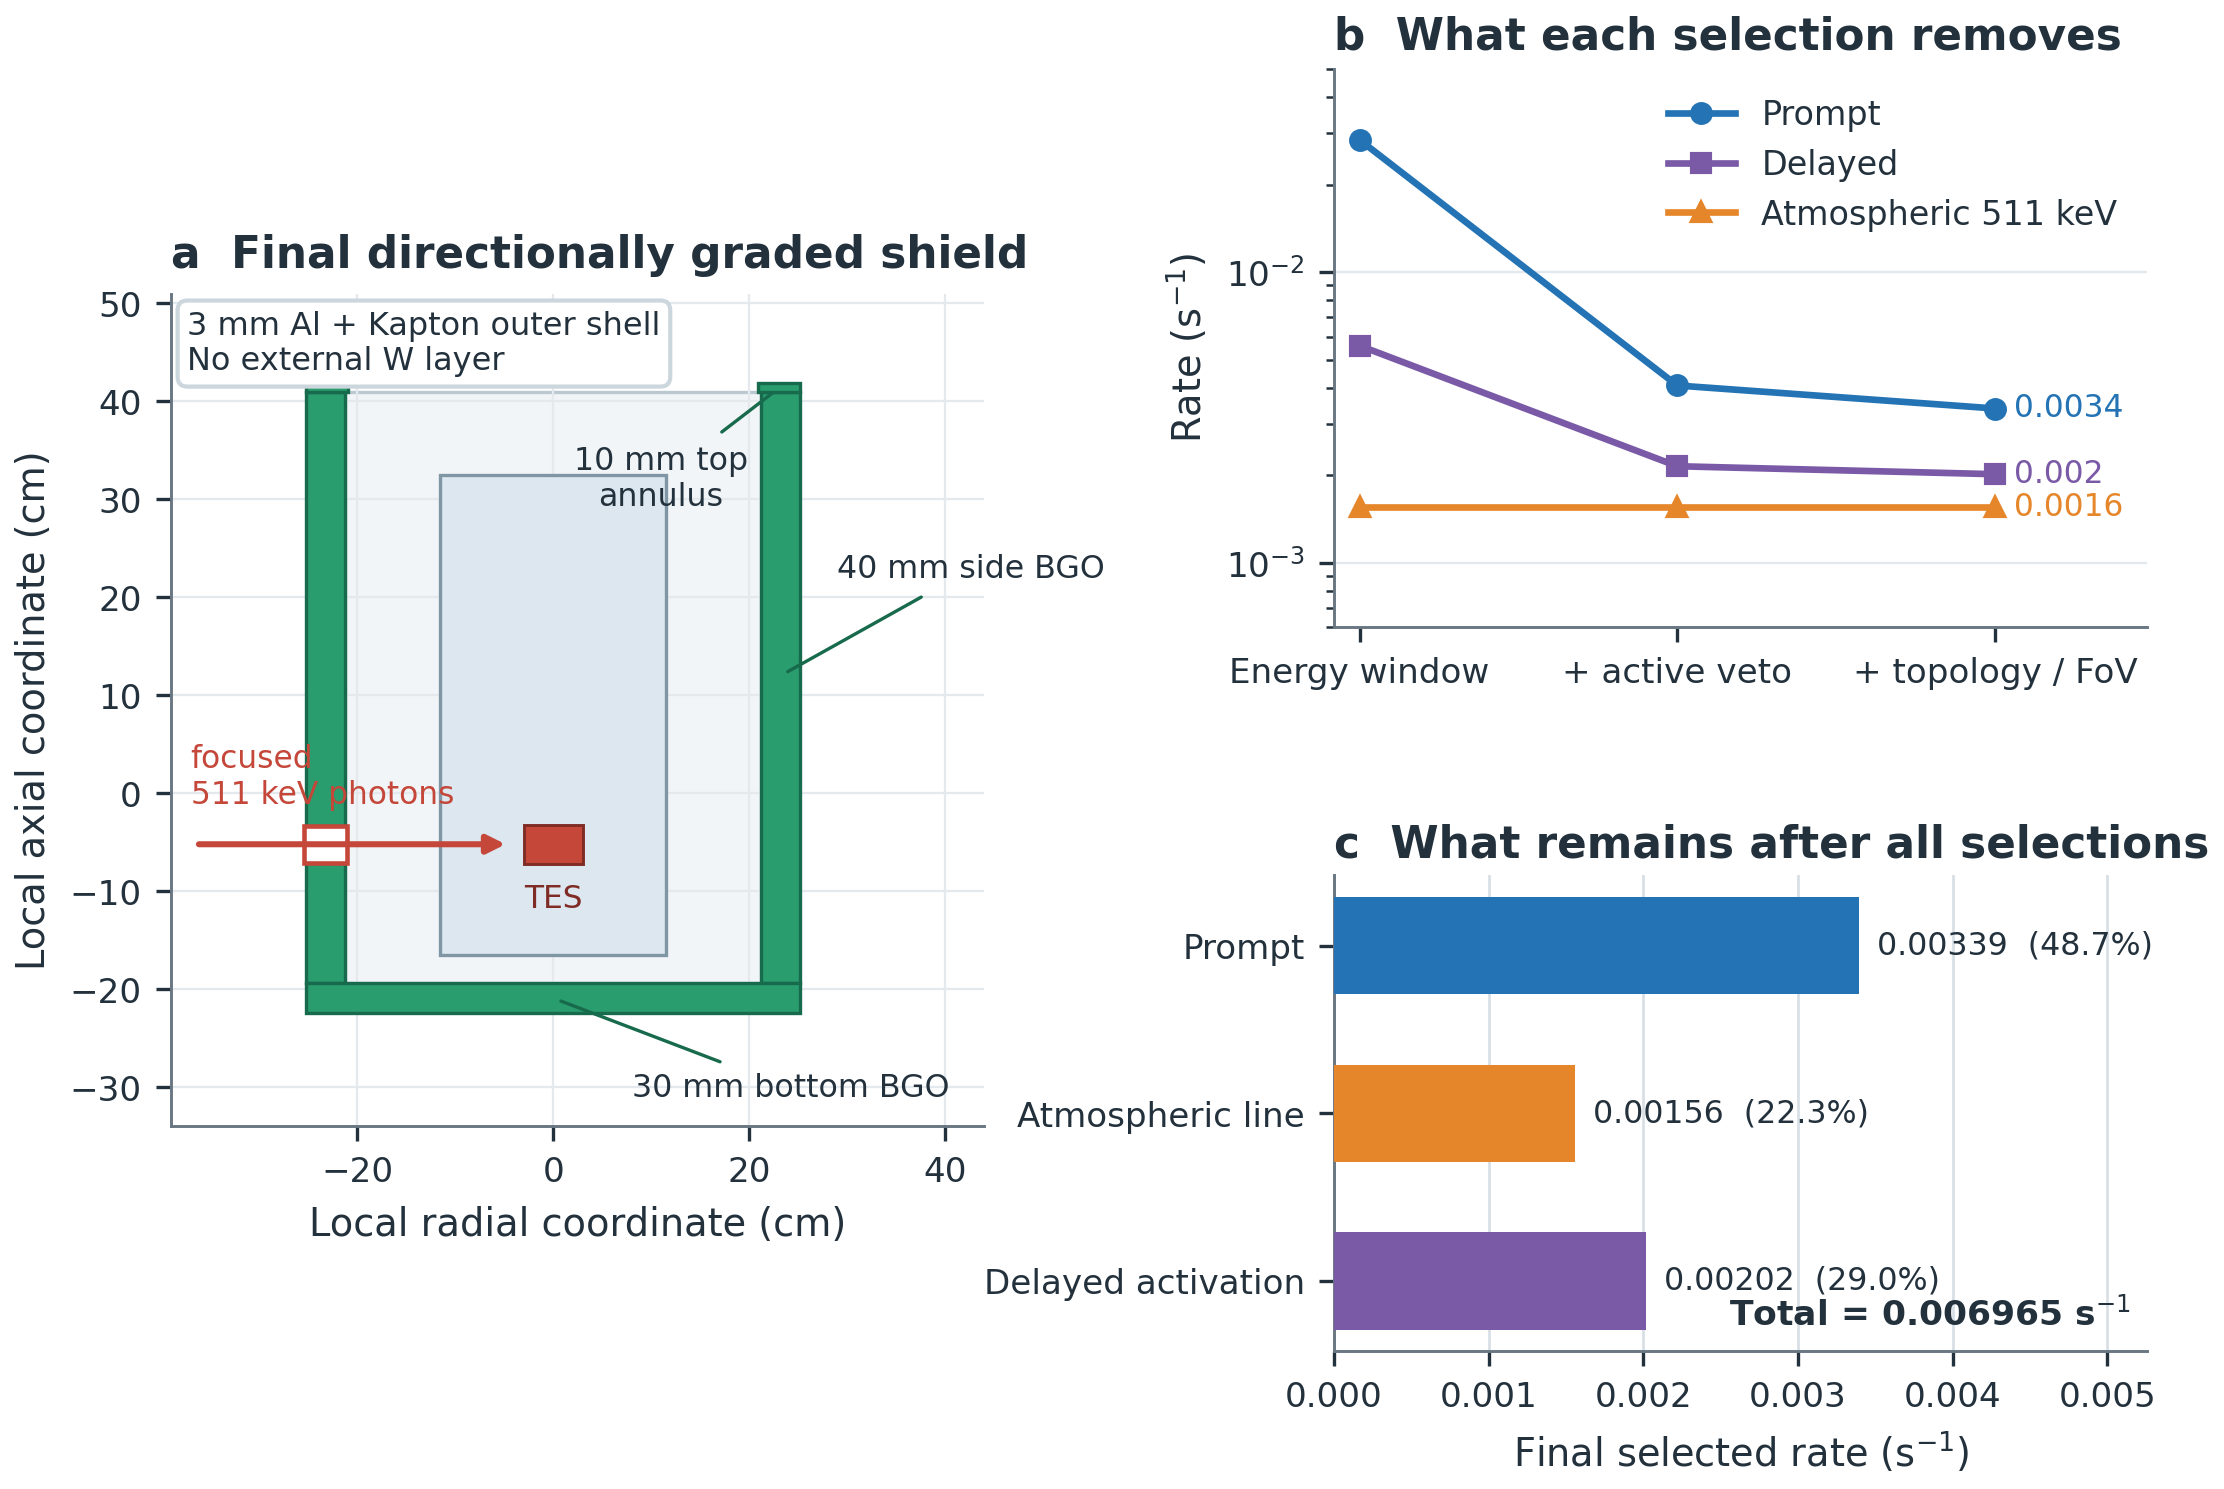
\includegraphics[width=0.90\linewidth]{paper_source_figure_table/fig_optimized_shield_background.png}
\caption{从最终方向分级屏蔽几何到选后本底。（a）方向分级 BGO 的截面，尺寸直接读取生成几何清单；为清楚展示屏蔽和侧入射光路，低温系统与 TES 符号作了简化。（b）瞬发、延迟和大气线在能窗、主动 veto、拓扑/视场选择后的率。（c）经能量响应卷积后最终 $6.96486\times10^{-3}\cps$ 本底的组成。}
\label{fig:optimized_shield_background_zh}
\end{figure}

\begin{table}[!ht]
\centering
\caption{最终方向分级主动屏蔽几何。径向与轴向坐标均位于探测器--低温系统局部坐标系。}
\label{tab:final_geometry_zh}
\footnotesize
\begin{tabular}{p{0.20\linewidth}p{0.34\linewidth}p{0.37\linewidth}}
\toprule
部件 & 最终设置 & 物理作用 \\
\midrule
侧 BGO & 40 mm；$r=21.2$--25.2 cm，$z=-19.4$--40.9 cm & 连续覆盖长侧壁，同时保留光学切口 \\
底部 BGO & 30 mm；$r=0$--25.2 cm，$z=-22.4$--$-19.4$ cm & 覆盖下端面 \\
顶部 BGO & 10 mm 环；$r=20.9$--25.2 cm，$z=40.9$--41.9 cm & 覆盖顶部外缘并保留中心服务开口 \\
侧入射光路 & 原有布尔孔、对准的 Al/Be 窗与 W 准直器 & 把聚焦 511 keV 光束送至 TES 阵列 \\
外部包络 & 3 mm Al 加 Kapton；无连续外部 W 层 & 机械包络与电绝缘 \\
BGO 离线反符合 & $E_{\mathrm{sh}}^{(c)}<50$ keV & 按事例汇总 BGO 主动体积中记录的能量沉积 \\
\bottomrule
\end{tabular}
\end{table}

这套屏蔽不是均匀厚度，而是把最深的主动层放在侧壁，在暴露路径较短的端面使用较小厚度。光学路径也保持清楚：W 准直器仍是束线上的局域元件，外部包络则不再增加第二层连续高原子序数材料。几何图、cut-flow 和分量预算因而是同一最终设计的三个相连视角。

\FloatBarrier

\subsection{全链本底与统计支撑}
\label{subsec:optimized_fullchain_zh}

表~\ref{tab:optimized_cutflow_zh} 按图~\ref{fig:optimized_shield_background_zh}b 的顺序跟踪最终几何中的每一条事例流。“预 veto”表示 TES 能量已经位于主线窗。记录数说明各阶段的 Monte Carlo 支撑；不同源流的曝光权重不同，最终带权率才是物理结果。

\begin{table}[!ht]
\centering
\caption{最终方向分级屏蔽几何在第 15 天参考状态经能量响应卷积后的主线窗 cut-flow。信号率按 $\fzero=10^{-4}\phcms$ 缩放；本底占比以最终总本底率为分母。}
\label{tab:optimized_cutflow_zh}
\footnotesize
\resizebox{\linewidth}{!}{%
\begin{tabular}{lrrrrrrr}
\toprule
流 & 预 veto 记录 & 主动 veto 后 & 最终记录 & 主动存活 / \% & 拓扑存活 / \% & 最终率 / $\cps$ & 本底占比 / \% \\
\midrule
八类瞬发 & 42 & 6 & 5 & 14.29 & 83.33 & $3.39303\times10^{-3}$ & 48.72 \\
全八族延迟 & 346 & 83 & 78 & 38.49 & 93.88 & $2.01657\times10^{-3}$ & 28.95 \\
大气 511\,keV 线 & 8 & 8 & 8 & 100.00 & 100.00 & $1.55526\times10^{-3}$ & 22.33 \\
聚焦信号 & 28566 & 28566 & 28010 & 100.00 & 98.05 & $9.86228\times10^{-4}$ & -- \\
\midrule
总本底 & 396 & 97 & 91 & -- & -- & $6.96486\times10^{-3}$ & 100.00 \\
\bottomrule
\end{tabular}}
\end{table}

主动屏蔽完成了大部分瞬发抑制：响应卷积后的线窗瞬发率由 $2.84914\times10^{-2}$ 降至 $4.07188\times10^{-3}\cps$，即只有 $14.29\%$ 通过主动 veto；拓扑/视场检验进一步把它降到 $3.39303\times10^{-3}\cps$。延迟活化在三个阶段的率依次为 $5.58116\times10^{-3}$、$2.14813\times10^{-3}$ 和 $2.01657\times10^{-3}\cps$。由于不同延迟族具有不同事例权重，表~\ref{tab:optimized_cutflow_zh} 中主动与拓扑存活率使用带权率之比（$38.49\%$ 与 $93.88\%$），而不是记录数之比。探测器响应卷积前有 9 条大气线输运记录位于主线窗；施加逐像素 420\,eV FWHM 响应和 0.3\,keV 测量命中阈值后，测量线窗内保留 8 条。本次响应实现中没有大气线像素命中被该阈值删除；一条事例在响应卷积后移至线窗下边界以下。线窗内 8 条记录均通过主动 veto 和拓扑检验，后两级选择中的率保持为 $1.55526\times10^{-3}\cps$；在本文采用的能量与拓扑观测量下，从开放光路进入的 511\,keV 光子与源光子不可区分。聚焦信号则不同：28566 条线窗记录全部通过主动 veto，最终有 28010 条（$98.05\%$）通过拓扑检验。

在第 15 天参考状态完成全部选择后，瞬发粒子占本底的 $48.72\%$，大气线占 $22.33\%$，延迟活化占 $28.95\%$。因此，主动 BGO 在保留聚焦束的同时去除了大多数带屏蔽沉积的瞬发和延迟事例；剩余本底自然分为瞬发漏过、线状大气项和局域活化三部分。

最终 5 条瞬发记录由 2 条 $e^+$ 和 3 条中子组成，其余六类瞬发粒子均为零条选后记录。表~\ref{tab:optimized_component_precision_zh} 保留这些零计数及其不同事例权重，因为零条记录给出的是率上限。光子族的单条权重最大，因而决定了条件式逐分量瞬发端点的大部分。

\begin{table}[!ht]
\centering
\caption{优化构型第 15 天最终本底的输运计数精度。对具有已定义输运曝光的分量，区间为双侧 95\% Garwood 区间乘以所列事例权重。小计和总计上端是逐分量端点之和，不是联合覆盖区间或探测器系统不确定度；有限 BUILDUP 为零的 $e^-$ 族不虚构曝光或 Garwood 端点。}
\label{tab:optimized_component_precision_zh}
\footnotesize
\resizebox{\linewidth}{!}{%
\begin{tabular}{lrrrrr}
\toprule
分量 & 最终记录 & 权重 / $\cps$ & 中心率 / $\cps$ & 精确 95\% 率区间 / $\cps$ & 中心总率占比 / \% \\
\midrule
瞬发 $\alpha$ & 0 & $6.78971\times10^{-4}$ & 0 & $[0,2.50464\times10^{-3}]$ & 0 \\
瞬发 $e^-$ & 0 & $6.78761\times10^{-4}$ & 0 & $[0,2.50387\times10^{-3}]$ & 0 \\
瞬发 $e^+$ & 2 & $6.78847\times10^{-4}$ & $1.35769\times10^{-3}$ & $[1.64423\times10^{-4},4.90446\times10^{-3}]$ & 19.49 \\
瞬发 $\gamma$ & 0 & $5.42680\times10^{-3}$ & 0 & $[0,2.00188\times10^{-2}]$ & 0 \\
瞬发 $\mu^-$ & 0 & $6.77164\times10^{-4}$ & 0 & $[0,2.49798\times10^{-3}]$ & 0 \\
瞬发 $\mu^+$ & 0 & $6.77705\times10^{-4}$ & 0 & $[0,2.49997\times10^{-3}]$ & 0 \\
瞬发 $n$ & 3 & $6.78446\times10^{-4}$ & $2.03534\times10^{-3}$ & $[4.19736\times10^{-4},5.94812\times10^{-3}]$ & 29.22 \\
瞬发 $p$ & 0 & $6.77234\times10^{-4}$ & 0 & $[0,2.49824\times10^{-3}]$ & 0 \\
瞬发小计 & 5 & -- & $3.39303\times10^{-3}$ & 上端之和：$4.33761\times10^{-2}$ & 48.72 \\
延迟 $\alpha$ & 1 & $3.48183\times10^{-7}$ & $3.48183\times10^{-7}$ & $[8.81522\times10^{-9},1.93995\times10^{-6}]$ & 0.005 \\
延迟 $e^-$ & 0 & -- & 0 & 有限 BUILDUP 零；无区间 & 0 \\
延迟 $e^+$ & 0 & $2.15006\times10^{-9}$ & 0 & $[0,7.93131\times10^{-9}]$ & 0 \\
延迟 $\gamma$ & 0 & $5.46390\times10^{-9}$ & 0 & $[0,2.01557\times10^{-8}]$ & 0 \\
延迟 $\mu^-$ & 5 & $4.20909\times10^{-6}$ & $2.10454\times10^{-5}$ & $[6.83339\times10^{-6},4.91130\times10^{-5}]$ & 0.30 \\
延迟 $\mu^+$ & 0 & $7.94287\times10^{-10}$ & 0 & $[0,2.93003\times10^{-9}]$ & 0 \\
延迟 $n$ & 60 & $3.28039\times10^{-5}$ & $1.96823\times10^{-3}$ & $[1.50197\times10^{-3},2.53351\times10^{-3}]$ & 28.26 \\
延迟 $p$ & 12 & $2.24533\times10^{-6}$ & $2.69439\times10^{-5}$ & $[1.39223\times10^{-5},4.70656\times10^{-5}]$ & 0.39 \\
延迟小计 & 78 & -- & $2.01657\times10^{-3}$ & 上端之和：$2.63166\times10^{-3}$ & 28.95 \\
大气 511\,keV 线 & 8 & $1.94408\times10^{-4}$ & $1.55526\times10^{-3}$ & $[6.71451\times10^{-4},3.06448\times10^{-3}]$ & 22.33 \\
\midrule
总本底 & 91 & -- & $6.96486\times10^{-3}$ & 逐分量上端：$4.90722\times10^{-2}$ & 100.00 \\
\bottomrule
\end{tabular}}
\end{table}

64 个确定性响应种子提供独立的数值积分检查。第 15 天本底的集合均值为
$6.94643\times10^{-3}\cps$、样本标准差为 $3.89046\times10^{-4}\cps$；预先固定的
主响应种子结果 $6.96486\times10^{-3}\cps$ 与均值相差 $0.047$ 个样本标准差。因此，
主结果采用该固定种子值，而响应种子集合不与表~\ref{tab:optimized_component_precision_zh}
的条件式逐分量输运计数端点混合。

\FloatBarrier

\subsection{最终几何的任务性能}
\label{subsec:final_mission_performance_zh}

最终选后率经过全部 81 个轨迹时间箱。偶然符合活时间因子保持在 0.97165--0.97985；到 20 d 时，中心曲线累计 1650.29 个聚焦信号计数和 11789.08 个本底计数，得到 $Z=15.199$。图~\ref{fig:optimized_mission_significance_zh} 展示显著度如何随时间积累，而不是只给终点。

\begin{figure}[!ht]
\centering
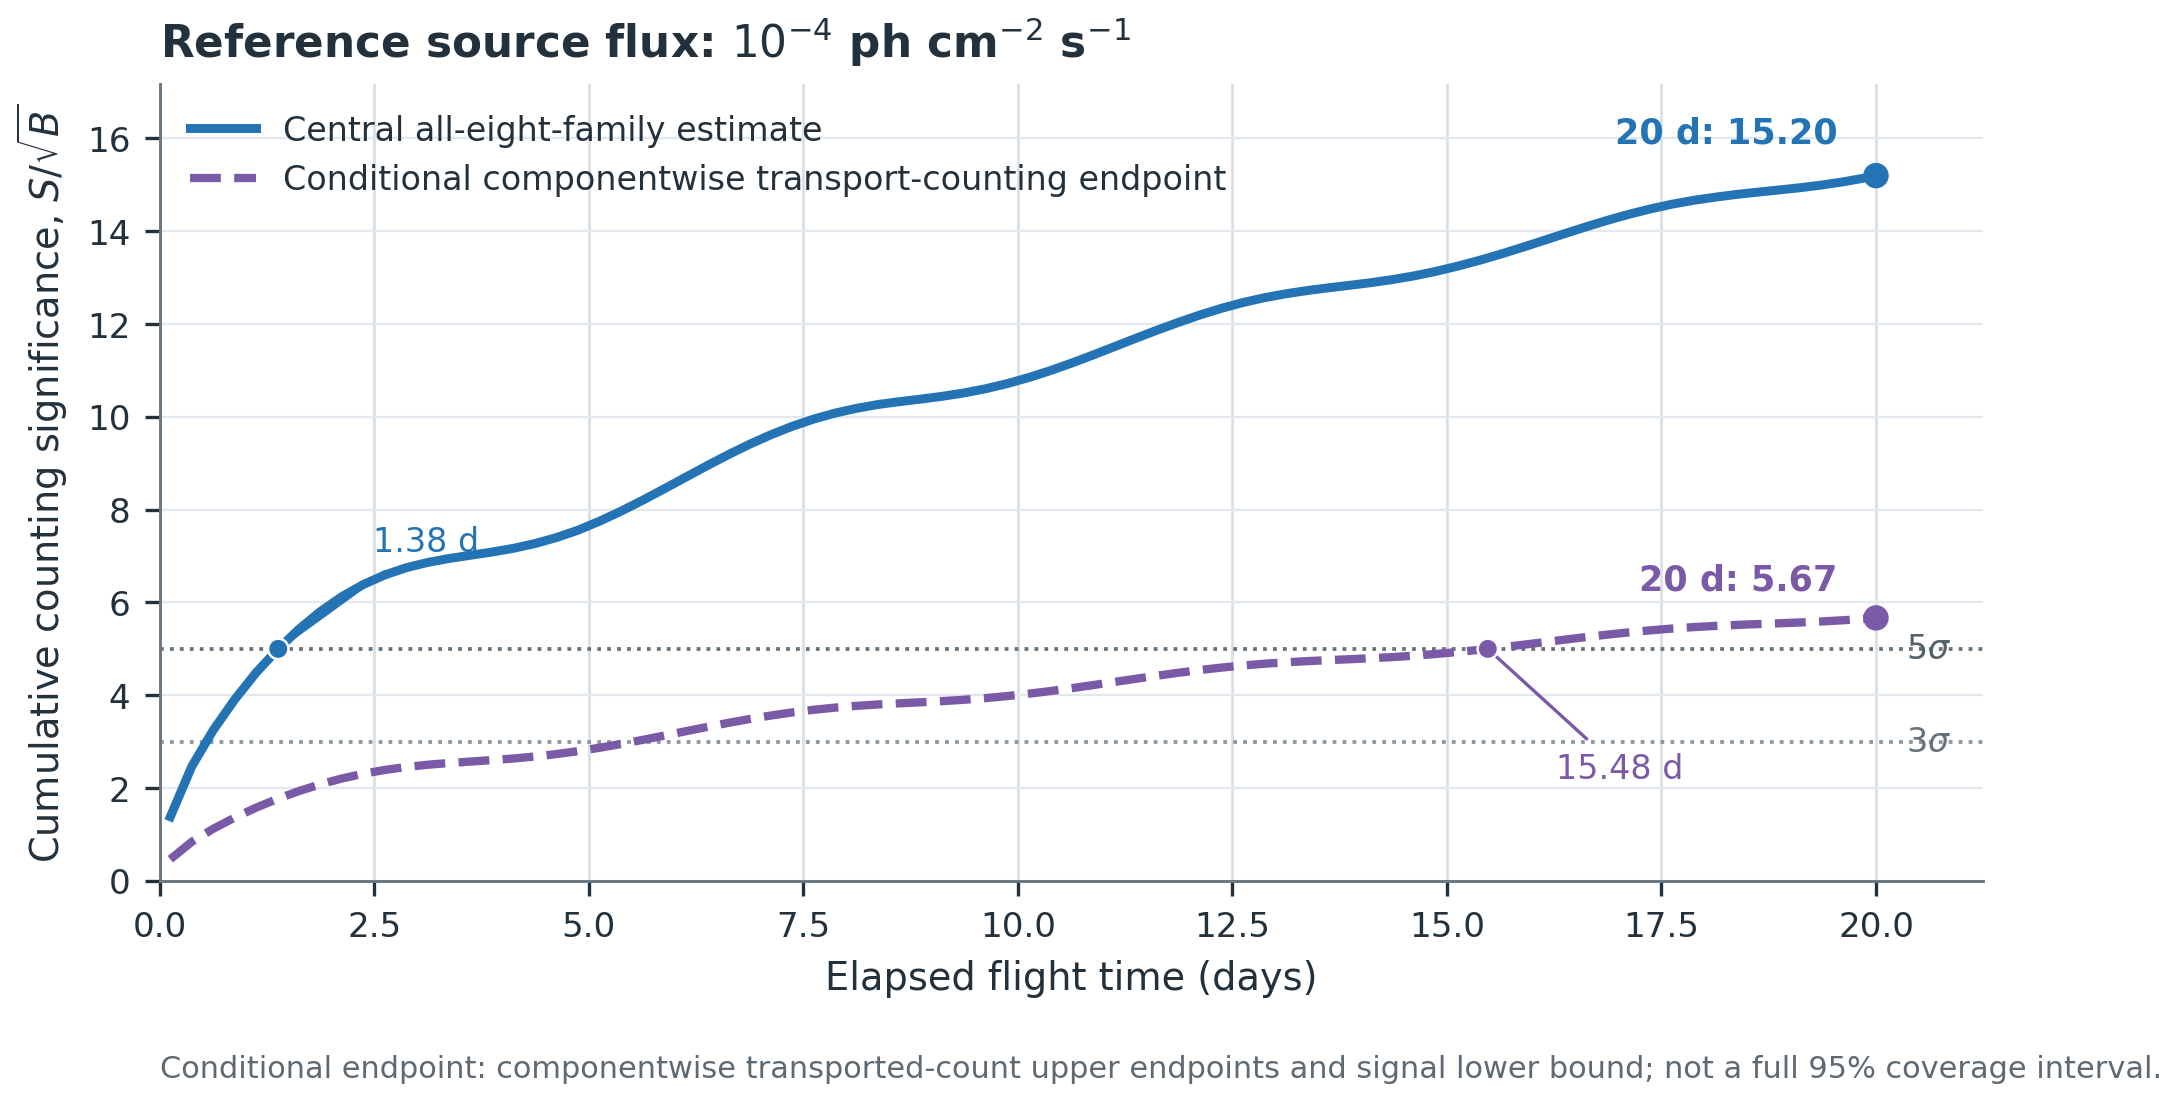
\includegraphics[width=0.98\linewidth]{paper_source_figure_table/fig_optimized_mission_significance.png}
\caption{最终方向分级屏蔽几何沿固定 $45^\circ$ 仰角的 20 d 参考轨迹连续观测大气层顶 $10^{-4}\phcms$ 点源时的累计计数显著度。实线使用能量响应卷积后的中心选后率；虚线对每个本底分量使用精确 95\% 计数上端，并对信号接受度使用精确 95\% 下端。其逐分量组合是条件式端点，不是联合 95\% 区间。两条曲线分别在 1.38 和 15.48 d 达到 $5\sigma$，20 d 时分别达到 15.20 和 5.67。}
\label{fig:optimized_mission_significance_zh}
\end{figure}

\begin{table}[!ht]
\centering
\caption{最终方向分级屏蔽几何的任务投影。端点列把逐分量 Garwood 本底上端和 Clopper--Pearson 信号下端经同一轨迹传播；它以已输运样本和选后“族--核素”混合为条件，不是联合覆盖区间。}
\label{tab:primary_sensitivity_zh}
\footnotesize
\begin{tabular}{lrr}
\toprule
量 & 中心估计 & 条件式逐分量输运计数端点 \\
\midrule
第 15 天本底 / $\cps$ & $6.96486\times10^{-3}$ & $4.90722\times10^{-2}$ \\
第 15 天 $\fzero$ 下信号 / $\cps$ & $9.86228\times10^{-4}$ & $9.80445\times10^{-4}$ \\
$T_{3\sigma}$ / d & 0.545 & 5.519 \\
$T_{5\sigma}$ / d & 1.382 & 15.476 \\
$Z_{20\mathrm{d}}$ & 15.199 & 5.667 \\
$\fthree(20\,\mathrm{d})$ / $\phcms$ & $1.9738\times10^{-5}$ & $5.2934\times10^{-5}$ \\
\bottomrule
\end{tabular}
\end{table}

两列回答两个直接问题。中心估计是当前模拟率的期望结果：0.545 d 达到 $3\sigma$，1.382 d 达到 $5\sigma$，20 d 的 $3\sigma$ 流量阈值为 $1.9738\times10^{-5}\phcms$。条件式端点把每个已输运本底分量推到精确计数上端，同时把信号接受度推到下端；它在 15.476 d 达到 $5\sigma$，20 d 阈值为 $5.2934\times10^{-5}\phcms$。该端点不具有 95\% 联合覆盖：逐分量上端之和没有联合覆盖保证，也不包括有限 BUILDUP 零族、有限 $M$ 源抽样和核素混合不确定度。两条曲线的大部分差距来自表~\ref{tab:optimized_component_precision_zh} 中零计数、高权重的瞬发光子分量，因此它也明确指出了增加哪一类 Monte Carlo 统计量最能提高预测精度。

\section{讨论}
\label{sec:discussion}

本文的主要结果，是用一条连续的物理链解释最终结构。在参考几何中，正电子和中子主导选后瞬发率；进入线窗的活化事例则来自 TES 附近的铜，而不是总活度最高的体积。最终方向分级屏蔽据此在侧向采用较厚 BGO，并把局域铜活化纳入同一事例选择。在第 15 天参考状态完成统一 veto 与拓扑检验后，本底为 $6.965\times10^{-3}\cps$，聚焦信号保留 $98.05\%$ 的线窗记录。几何、本底预算和任务曲线因此是同一结果的三个视角。

这一分析顺序与近期仪器本底研究采用的方法一致。COSI 从实际载荷模型出发，分开瞬发和活化分量，再把能谱与时间变化同飞行数据比较 \cite{Gallego2025Balloon}；DIXE 也先建立详细 TES 载荷模型，再追问哪些入射粒子、产生区域和过程构成探测谱 \cite{Tian2026DIXE}。本文的分解尤其重要，因为源清单与线窗选后本底给出不同答案：参考活度由 $^{128}$I 主导，选后延迟记录却由冷铜核素主导。以选后事例而不是总活度驱动设计，能够让优化始终围绕科学能窗。

最终分量组成也显示每一层仪器选择的作用。主动 BGO 去除了大部分伴随屏蔽沉积的瞬发与延迟事例；拓扑检验提供较小的额外抑制，同时几乎保留全部聚焦事例。大气 511 keV 分量仍然保留，是因为它在当前能量与单光子拓扑观测量中可与天体源事例简并。它在第 15 天参考状态占本底的 $22.33\%$；这一残余并非反符合失效，而是需要沿轨迹保留的方向相关全空间大气线本底。它能否与源辐射分离，仍需在后续指向和控制区分析中检验。

该望远镜的观测角色与 INTEGRAL/SPI、COSI 对弥散核球、银盘和更广银河辐射的测量互补 \cite{Siegert2016AA,Kierans2020,Siegert2020COSI,Yoneda2025,Karwin2023}。Laue 透镜 TES 概念以视场换取集中束流和亚 keV 线窗，自然适用于紧凑 511 keV 源、未分辨中央成分和指向式后随观测。表~\ref{tab:primary_sensitivity_zh} 的 20 d 数值对应的正是这种连续在源的窄线参考情形。

\subsection{适用范围与下一步}
\label{subsec:limitations}

任务数值是对工程探测器--低温系统几何和连续在源合成轨迹的统计投影。计算采用 50 keV 的 BGO 离线沉积能 veto，并使用探测器层拓扑检验以及最终延迟流中的全八族活化；其中 7 族具有正活度延迟输运，$e^-$ 是有限 BUILDUP 零观测而非物理零声明。veto 在后处理中施加于逐事例汇总的屏蔽沉积。该判据是理想沉积能阈值，而非由 BGO 硬件触发效率曲线建模得到的阈值。当前本底预算仅涵盖探测器--低温系统质量模型，不包括 Laue 光学系统和气球平台产生的本底。这些设置定义了中心曲线和条件式逐分量输运计数端点所代表的计算；后者既不是联合 95\% 覆盖区间，也不涵盖辐射场、截面、有限 $M$、核素混合、标定和重建系统学。

大气线分量还具有独立的源模型限制。本文结果采用第~\ref{subsec:atm511_source_zh}~小节的名义归一化、截止刚度与深度标度以及半经验下行角分布。EXPACS/PARMA 平滑连续谱未作线成分扣除，因此它与独立大气线之间的未解析重叠是已识别但尚未量化的源模型不确定度。任务折叠仅缩放总线通量并保留第 15 天已输运的角响应，没有在每个时间箱重新运行 Cosima。这些因素未计入条件式逐分量输运计数端点。

下一步可以集中在图中最有影响的项：提高决定条件式端点的瞬发光子曝光，重复全族活化产生位置抽样以量化有限 $M$ 收敛，用具体飞行计划和可见度历史替换参考轨迹，并在最终探测器设计上标定能量响应与 veto 阈值。随后可用空间--谱联合似然利用聚焦斑和控制区，同时对本底扰动参数做剖面 \cite{Cowan2011}。这一路径扩展当前分量模型，而不改变其“源--材料--事例--几何”的主线。

\subsection{结论}
\label{sec:conclusions}

质量完备参考几何清楚显示聚焦束、TES 阵列、冷铜和主动屏蔽如何相交。选后事例图把正电子和中子识别为主要瞬发来源，把冷铜核素识别为延迟线窗来源；这些信息导向侧/底/顶 40/30/10 mm BGO 的最终方向分级屏蔽。第 15 天参考状态的最终几何全链在大气层顶 $\fzero=10^{-4}\phcms$ 下给出 $B=6.965\times10^{-3}\cps$ 和 $S=9.862\times10^{-4}\cps$。沿固定 $45^\circ$ 仰角的 20 d 参考轨迹，中心与条件式逐分量输运计数结果分别达到 $Z=15.20$ 和 5.67，对应的 $3\sigma$ 阈值为 $1.974\times10^{-5}$ 和 $5.293\times10^{-5}\phcms$。这说明，按粒子和材料追溯的本底模型可以直接转化为清楚的最终几何与任务尺度 511 keV 性能预测。

\section*{数据与软件可用性}
正式发表前，应通过带版本号的公共代码仓库或机构存档提供复现本文图表所需的几何和源定义、随机种子、分析与制图脚本、LaTeX 源文件及派生验证产物。

\section*{声明}
\textbf{经费来源} 投稿前补充。

\textbf{利益冲突} 投稿前补充。

\textbf{作者贡献} 投稿前补充。

\textbf{伦理审批与参与同意} 不适用。

\begin{thebibliography}{99}

\bibitem{Prantzos2011}
N. Prantzos, C. Boehm, A.M. Bykov, R. Diehl, K. Ferriere, N. Guessoum, P. Jean, J. Knoedlseder, A. Marcowith, I.V. Moskalenko, A. Strong, G. Weidenspointner, The 511 keV emission from positron annihilation in the Galaxy, Rev. Mod. Phys. 83 (2011) 1001--1056, doi:10.1103/RevModPhys.83.1001.

\bibitem{Jean2006}
P. Jean, J. Knoedlseder, V. Lonjou, M. Allain, J.-P. Roques, G.K. Skinner, B.J. Teegarden, G. Vedrenne, P. von Ballmoos, B. Cordier, P. Caraveo, R. Diehl, P. Durouchoux, P. Leleux, R. Schanne, G. Weidenspointner, Spectral analysis of the Galactic $e^+e^-$ annihilation emission, Astron. Astrophys. 445 (2006) 579--589, doi:10.1051/0004-6361:20053765.

\bibitem{Kierans2020}
C.A. Kierans, S.E. Boggs, A. Zoglauer, A.W. Lowell, C. Sleator, J. Beechert, T.J. Brandt, P. Jean, H. Lazar, J. Roberts, T. Siegert, J.A. Tomsick, P. von Ballmoos, Detection of the 511 keV Galactic positron annihilation line with COSI, Astrophys. J. 895 (2020) 44, doi:10.3847/1538-4357/ab89a9.

\bibitem{Siegert2016AA}
T. Siegert, R. Diehl, G. Khachatryan, M.G.H. Krause, F. Guglielmetti, J. Greiner, A.W. Strong, X. Zhang, Gamma-ray spectroscopy of positron annihilation in the Milky Way, Astron. Astrophys. 586 (2016) A84, doi:10.1051/0004-6361/201527510.

\bibitem{Siegert2016V404}
T. Siegert, R. Diehl, J. Greiner, M.G.H. Krause, A.M. Beloborodov, M. Cadolle Bel, F. Guglielmetti, J. Rodriguez, A.W. Strong, X. Zhang, Positron annihilation signatures associated with the outburst of the microquasar V404 Cygni, Nature 531 (2016) 341--343, doi:10.1038/nature16978.

\bibitem{Knodlseder2005AllSky}
J. Knoedlseder, P. Jean, V. Lonjou, G. Weidenspointner, N. Guessoum, R. Diehl, W. Gillard, M.J. Harris, G.K. Skinner, P. von Ballmoos, G. Vedrenne, P. Caraveo, B. Cordier, V. Schoenfelder, B.J. Teegarden, The all-sky distribution of 511 keV electron-positron annihilation emission, Astron. Astrophys. 441 (2005) 513--532, doi:10.1051/0004-6361:20042063.

\bibitem{Yoneda2025}
H. Yoneda, T. Siegert, S. Mittal, Imaging the positron annihilation line with 20 years of INTEGRAL/SPI observations, arXiv:2509.01066, 2025.

\bibitem{Siegert2020COSI}
T. Siegert, S.E. Boggs, J.A. Tomsick, A.C. Zoglauer, C.A. Kierans, C.C. Sleator, J. Beechert, T.J. Brandt, P. Jean, H. Lazar, A.W. Lowell, J.M. Roberts, P. von Ballmoos, Imaging the 511 keV positron annihilation sky with COSI, Astrophys. J. 897 (2020) 45, doi:10.3847/1538-4357/ab9607.

\bibitem{Siegert2019Kinematics}
T. Siegert, R. Diehl, G. Khachatryan, M.G.H. Krause, F. Guglielmetti, J. Greiner, A.W. Strong, X. Zhang, Constraints on positron annihilation kinematics in the inner Galaxy, Astron. Astrophys. 627 (2019) A126, doi:10.1051/0004-6361/201833856.

\bibitem{DeCesare2011}
G. De Cesare, Searching for the 511 keV annihilation line from galactic compact objects with the IBIS gamma ray telescope, Astron. Astrophys. 531 (2011) A56, doi:10.1051/0004-6361/201116516.

\bibitem{Barriere2009Laue}
N.M. Barriere, L. Natalucci, N. Abrosimov, P. von Ballmoos, P. Bastie, P. Courtois, M. Jentschel, J. Knodlseder, J. Rousselle, P. Ubertini, Soft gamma-ray optics: new Laue lens design and performance estimates, arXiv:0910.0488, 2009.

\bibitem{Barriere2011LauePrototype}
N.M. Barriere, J.A. Tomsick, S.E. Boggs, A. Lowell, P. von Ballmoos, Developing a second generation Laue lens prototype: high reflectivity crystals and accurate assembly, arXiv:1111.6700, 2011.

\bibitem{Weidenspointner2006MAX}
G. Weidenspointner, C.B. Wunderer, N. Barriere, A. Zoglauer, P. von Ballmoos, Monte Carlo study of detector concepts for the MAX Laue Lens gamma-ray telescope, arXiv:astro-ph/0603152, 2006.

\bibitem{Shirazi2023}
F. Shirazi, E. Gau, M.A. Hossen, D. Becker, D. Schmidt, D. Swetz, D. Bennett, D. Braun, F. Kislat, J. Gard, J. Mates, J. Weber, N.R. Cavero, S. Chun, L. Lisalda, A. West, B. Dev, F. Ferrer, R. Bose, J. Ullom, H. Krawczynski, The 511-CAM Mission: A pointed 511 keV gamma-ray telescope with a focal plane detector made of stacked transition edge sensor microcalorimeter arrays, J. Astron. Telesc. Instrum. Syst. 9 (2023) 024006, doi:10.1117/1.JATIS.9.2.024006.

\bibitem{Zhang2022TESGamma}
S. Zhang, J.-K. Xia, T. Sun, et al., Transition edge sensor based detector: from X-ray to gamma-ray, arXiv:2204.00010, 2022.

\bibitem{Hu2026}
K. Hu, M. Fritts, D. Becker, D. Schmidt, F. Zhou, A. Dasgupta, F. Kislat, M. Keller, S. Chun, A.G. Detoito, E. Gau, X. Jin, D. Bennett, D. Braun, J. Gard, J.A.B. Mates, J. Nobles, D. Radomski, N. Rodriguez Cavero, R. Snodgrass, D. Swetz, J. Ullom, S. Vengalil Menon, J. Weber, K. Wimalasena, H. Krawczynski, Design of a mission to measure the shape and substructure of the 511 keV gamma-ray line from the center of the Milky Way, J. Astron. Telesc. Instrum. Syst. 12 (2026) 025002, doi:10.1117/1.JATIS.12.2.025002.

\bibitem{Gallego2025Balloon}
S. Gallego, U. Oberlack, J. Lommler, C.M. Karwin, A. Zoglauer, P. Jean, P. von Ballmoos, C. Kierans, C.C. Sleator, J.A. Tomsick, S.E. Boggs, Bottom-up background simulations of the 2016 COSI balloon flight, Astrophys. J. 986 (2025) 116, doi:10.3847/1538-4357/add6a0.

\bibitem{Tian2026DIXE}
R. Tian, J. Mao, J. Liu, H. Jin, W. Cui, Simulation of non-X-ray background for the DIffuse X-ray Explorer (DIXE) mission, arXiv:2604.13569, 2026.

\bibitem{Caputo2017}
R. Caputo, F. Kislat, J. Racusin, on behalf of the AMEGO Team, AMEGO: Simulations of the instrument performance, Proc. 35th International Cosmic Ray Conference, PoS(ICRC2017) 783 (2018), doi:10.22323/1.301.0783.

\bibitem{Gottardi2021TESReview}
L. Gottardi, K. Nagayoshi, A review of X-ray microcalorimeters based on superconducting transition edge sensors for astrophysics and particle physics, Applied Sciences 11 (2021) 3793, doi:10.3390/app11093793.

\bibitem{Xie2026AlMn}
L. Xie, Y. Zhang, Z. Li, Z. Liu, S. Shu, J. Zhou, X. Li, H. Li, H. Gao, Y. Gu, X. Lu, Y. Zhao, C. Liu, Beyond one-thousandth energy resolution with an AlMn TES detector, arXiv:2602.11728, 2026.

\bibitem{Vavagiakis2017AlMnMagnetic}
E.M. Vavagiakis, S.W. Henderson, K. Zheng, H.-M. Cho, N.F. Cothard, B. Dober, S.M. Duff, P.A. Gallardo, G. Hilton, J. Hubmayr, K.D. Irwin, B.J. Koopman, D. Li, F. Nati, M.D. Niemack, C.D. Reintsema, S. Simon, J.R. Stevens, A. Suzuki, B. Westbrook, Magnetic sensitivity of AlMn TESes and shielding considerations for next-generation CMB surveys, arXiv:1710.08456, 2017.

\bibitem{NISTXCOM}
J.H. Hubbell, S.M. Seltzer, XCOM: Photon Cross Section Database, NIST Standard Reference Database 8 (XGAM), National Institute of Standards and Technology, doi:10.18434/T48G6X.

\bibitem{Sturner2003}
S.J. Sturner, C.R. Shrader, G. Weidenspointner, B.J. Teegarden, D. Attie, B. Cordier, R. Diehl, C. Ferguson, P. Jean, A. von Kienlin, P. Paul, F. Sanchez, S. Schanne, P. Sizun, G. Skinner, C.B. Wunderer, Monte Carlo simulations and generation of the SPI response, Astron. Astrophys. 411 (2003) L81--L84, doi:10.1051/0004-6361:20031171.

\bibitem{Agostinelli2003}
S. Agostinelli, J. Allison, K. Amako, et al., Geant4---a simulation toolkit, Nucl. Instrum. Methods Phys. Res. A 506 (2003) 250--303, doi:10.1016/S0168-9002(03)01368-8.

\bibitem{Allison2016}
J. Allison, K. Amako, J. Apostolakis, et al., Recent developments in Geant4, Nucl. Instrum. Methods Phys. Res. A 835 (2016) 186--225, doi:10.1016/j.nima.2016.06.125.

\bibitem{SanchezDelRio2011XOP}
M. Sanchez del Rio, R.J. Dejus, XOP v2.4: recent developments of the x-ray optics software toolkit, Proc. SPIE 8141 (2011) 814115, doi:10.1117/12.893911.

\bibitem{Guan2023BraggReflection}
F. Guan, M. Asai, D.A. Bartkoski, M. Kleckner, Z. Harel, M. Salehpour, Adding the X-ray Bragg reflection physical process in crystal to the Geant4 Monte Carlo simulation toolkit, part I: reflection from a crystal slab, Precision Radiation Oncology 7(1) (2023) 59--66.

\bibitem{Reiazi2025G4BraggReflection}
R. Reiazi, D. Lee, D. Bartkoski, M. Kleckner, M. Salehpour, G4BraggReflection for accurate modeling of Bragg reflection in perfect and mosaic crystals, J. Phys. D: Appl. Phys. 58 (2025) 295102, doi:10.1088/1361-6463/aded1d.

\bibitem{Zoglauer2006}
A. Zoglauer, R. Andritschke, F. Schopper, MEGAlib: The Medium Energy Gamma-ray Astronomy Library, New Astron. Rev. 50 (2006) 629--632, doi:10.1016/j.newar.2006.06.049.

\bibitem{Sato2015EXPACS}
T. Sato, Analytical model for estimating terrestrial cosmic ray fluxes nearly anytime and anywhere in the world: extension of PARMA/EXPACS, PLoS ONE 10 (2015) e0144679, doi:10.1371/journal.pone.0144679.

\bibitem{Sato2016PARMA4}
T. Sato, Analytical model for estimating the zenith angle dependence of terrestrial cosmic ray fluxes, PLoS ONE 11 (2016) e0160390, doi:10.1371/journal.pone.0160390.

\bibitem{Mahoney1981Atmospheric}
W.A. Mahoney, J.C. Ling, A.S. Jacobson, HEAO 3 measurements of the atmospheric positron annihilation line, J. Geophys. Res. 86 (1981) 11098--11104, doi:10.1029/JA086iA13p11098.

\bibitem{Harris2003Atmospheric}
M.J. Harris, G.H. Share, M.D. Leising, Spatial and temporal variability of the gamma radiation from Earth's atmosphere during a solar cycle, J. Geophys. Res. Space Phys. 108 (2003) 1435, doi:10.1029/2003JA009958.

\bibitem{Kondev2021NUBASE}
F.G. Kondev, M. Wang, W.J. Huang, S. Naimi, G. Audi, The NUBASE2020 evaluation of nuclear physics properties, Chinese Phys. C 45 (2021) 030001, doi:10.1088/1674-1137/abddae.

\bibitem{Kierans2017}
C.A. Kierans, S.E. Boggs, J.-L. Chiu, A. Lowell, C. Sleator, J.A. Tomsick, A. Zoglauer, M. Amman, H.-K. Chang, C.-H. Tseng, C.-Y. Yang, C.-H. Lin, P. Jean, P. von Ballmoos, The 2016 Super Pressure Balloon flight of the Compton Spectrometer and Imager, arXiv:1701.05558, 2017.

\bibitem{Karwin2023}
C.M. Karwin, T. Siegert, J. Beechert, J.A. Tomsick, T.A. Porter, M. Negro, C. Kierans, M. Ajello, I. Martinez Castellanos, A. Shih, A. Zoglauer, S.E. Boggs, Probing the Galactic diffuse continuum emission with COSI, arXiv:2310.12206, 2023.

\bibitem{Cowan2011}
G. Cowan, K. Cranmer, E. Gross, O. Vitells, Asymptotic formulae for likelihood-based tests of new physics, Eur. Phys. J. C 71 (2011) 1554, doi:10.1140/epjc/s10052-011-1554-0.

\end{thebibliography}
\end{document}
